\documentclass{rspublic}   

%------------------------------------------------------------------------- 
% take the % away on next line to produce the final camera-ready version 
%\pagestyle{empty}

%\usepackage[utf8]{inputenc}
\usepackage{graphicx}
\usepackage{url}
\usepackage{float}
\usepackage{times}    
\usepackage{multirow}    
\usepackage{listings}   
\usepackage{times}     
\usepackage{paralist}    
\usepackage{wrapfig}    
\usepackage[small,it]{caption}
\usepackage{multirow}
\usepackage{ifpdf}   
\usepackage{subfigure} 

                    
%Bibliography                     
\usepackage{natbib}   

\usepackage{listings}
\usepackage{keyval}  
\usepackage{color}
\definecolor{listinggray}{gray}{0.95}
\definecolor{darkgray}{gray}{0.7}
\definecolor{commentgreen}{rgb}{0, 0.4, 0}
\definecolor{darkblue}{rgb}{0, 0, 0.4}
\definecolor{middleblue}{rgb}{0, 0, 0.7}
\definecolor{darkred}{rgb}{0.4, 0, 0}
\definecolor{brown}{rgb}{0.5, 0.5, 0}

\title[Efficient Large-Scale Replica-Exchange Simulations on
Production Infrastructure]{Efficient Large-Scale Replica-Exchange
  Simulations on Production Infrastructure}

\author[Thota, Luckow, Jha]{
  Abhinav Thota$^{1,2}$, Andr\'e Luckow$^{1}$ and Shantenu Jha$^{1,3}$\\
  \small{\emph{$^{1}$Center for Computation \& Technology, Louisiana
      State University, Baton Rouge, LA 70803, USA}}
   \small{\emph{$^{2}$Department of Computer Science, Louisiana State
        University, Baton Rouge, LA 70803, USA}}\\
    \small{\emph{$^{3}$ Rutgers, State University of New Jersey}}}

%\date{}

\def\acknowledgementname{Acknowledgements}
\newenvironment{acknowledgement}%
{\section*{\acknowledgementname}%
\parindent=0pt%
}

\newif\ifdraft
%\drafttrue
\ifdraft
\newcommand{\jhanote}[1]{ {\textcolor{red} { ***shantenu: #1 }}}
\newcommand{\alnote}[1]{ {\textcolor{blue} { ***andre: #1 }}}
\newcommand{\athotanote}[1]{ {\textcolor{green} { ***athota: #1 }}}
\else
\newcommand{\alnote}[1]{}
\newcommand{\athotanote}[1]{}
\newcommand{\jhanote}[1]{}
\fi

\newcommand{\I}[1]{\textit{#1}}
\newcommand{\B}[1]{\textbf{#1}}
\newcommand{\T}[1]{\texttt{#1}}

\newcommand{\glidein}[1]{Glide-In }  
\newcommand{\ReplicaAgent}[1]{Replica-Agent }         
\newcommand{\replicaagent}[1]{replica-agent }         
\newcommand{\remanager}[1]{RE-Manager }
\begin{document} 
\maketitle    

%   The design and development of an application is often influenced and
%   constrained by the programming systems and the infrastructure it is
%   developed against.  It is important to break the coupling between
%   the development and the underlying infrastructure, in order to
%   enable applications to be flexible (across infrastructure),
%   extensible (to new methods of communication and coordination) and
%   scalable.
  % Developing applications that are able to orchestrate
%   heterogeneous resources across distributed resources is a complex
%   task yet is an important design objective of both logically and
%   physically distributed applications. 

\begin{abstract}{Replica-Exchange, SAGA, Large-Scale, Production}
  Replica-Exchange (RE) algorithms are used to understand physical
  phenomena -- ranging from protein folding dynamics to binding
  affinity calculations.  They represent a class of algorithms that
  involve a large number of loosely-coupled ensembles, and are thus
  amenable to using distributed resources. We develop a framework for
  RE which supports different replica pairing (synchronous vs.
  asynchronous) and exchange coordination mechanisms (centralised vs.
  decentralised) and which can use a range of production
  cyberinfrastructure concurrently.  We characterise the performance
  of both RE algorithms at unprecedented number of cores employed --
  the number of replicas and the typical number of cores per replica -- on
  production distributed infrastructure.  We find that the
  asynchronous algorithms outperform the synchronous algorithm, even
  though details of the specific implementations are important
  determinants of performance.

\end{abstract}
% \alnote{We are on about 13.5 pages (without comments). 
% Do we need to shorten it to 12? space-saving? Or is it sufficient
% to do it with the camera-ready version?}


%\athotanote{addressed: corrected graph: from no. replicas to no. machines. 8. It seems that even in the decentralized case, the advert service is still centralized? Are there issues of latency when accessing the advert service or keeping it consistent? 9. When multiple replicas are concurrently searching for a partner to exchange with it is not clear how this is done safely. Even with reverification non-deterministic behavior could still arise if care is not taken. 7. In section 3b(ii) -- what is "MD"? - we explain this earlier as molecular dynamics in parenthesis.. should we do that again? - fixed 6. The advert service (in section 3(a)) needs further discussion. What is an advert in this context. Also how is a key/value pair generated. What does it mean in this context. Is this similar to a DHT in a peer-2-peer system? In particular, the authors should explain how a job is described -- and subsequently matched. 4. The time calculation in equation 2.2 needs further elaboration. Parameters such as T-ex, T-mgmt are not clear. For instance, the mention of an "advert-server" is surely an implementation detail? (corrected) In particular, the authors should comment on whether such a simple linear combination is an effective representation of reality -- given that many of these operations are being performed over a distributed environment. - addressed in section 2(a) 3. It would be useful for the authors to compare the replica exchange application, as disussed here, with the general class of "parameter sweep" application -- where some synchronisation may also be required. - addressed in section 2(b) 2. There needs to be an explanation of why the temperature needs to be exchanged between replicas and what the role of the Metropolis algorithm is. 5. What is the "Metropolis scheme" -- give reference or explain.- we reference metropolis in section 2.  1. The paper would be improved if the work were better motivated by an example application near the start of the paper (for example, the MD simulation that is used later in the paper) - in introduction. 1) Don't use symbols to refer to "Section" - write it out as text. 2) Try to avoid using the word "utilize" and derivatives thereof. The word "use" can almost always be used instead. 3) Introduction, line 1, change to "Replica-Exchange (RE)......methods represent a class of algorithms..." 4) Introduction, first para: Change "developed against" to "developed within"? 5) Introduction, near end of second para: remove "different coordination mechanisms". 6) Section 2(a), line 3: change to "total time-to-completion of an experiment". 7) Don't use ampersand - use "and" instead. 8) 3 lines after eqn. 2.2: this is the first mention of the advert server, so you either need to explain what it is, or make a forward reference, or drop the text in parentheses. Also "book-keeping" should be "bookkeeping". 9) Last line of page 2: change to "in the asynchronous-centralised case". 10) Section 2(b), second para, line 1: change to "For the synchronous RE formulation". 11) Section 2(b), third para: omit comma after "consequence". 12) Section 2(b), fourth para, line 1: omit "there are". 13) Section 3(a), first para, last line: change "the conduction of" to "conducting". 14) Section 3(a), second para, line 2: change to "enables the dynamical use of a range of" 15) Section 3(a), third para, change "store which is used for" to "store used for". 16) Section 3(a), third para, line 6: change to "multiple big-jobs". 17) Section 3(b), second para, line 5: change to "has a centralised". 18) Section 3(b)(ii), second para, line 6/7: change to "still in the done state". 19) Section 4, first para, line 3: change to "as well as a basic" 20) Section 4(b), first para, line 2: change to "is in the synchronisation" 21) Section 4(b), third para, line 9: change to "suggests there are between 2 and 4" 22) Section 4(b), third para, line 11: change to "increasing numbers of replicas". 23) Section 4(c), first para, last line: change to "in these cases" 24) Section 5(a), first para, last line: "the" is repeated" 25) Section 5(a), second para, line 2: change to "exchanges to replicas" 26) Section 5(a), last para, last line: "the" is repeated" 27) Section 5(b), first para, line 1: change to "of the asynchronous" 28) Section 6, first para, line 1: change to "Following theoretical underpinnings (Li and Parashar 2007, Gallicchio et al. 2008), in this paper..." 29) Section 6, second para, line 2: change "enable" to "enables" 30) Section 6, second para, line 5: change "out weight" to "outweigh".}


\section{Introduction}

Replica-Exchange (RE)~\citep{hansmann,Sugita:1999rm} methods have been
used to understand physical phenomena -- ranging from protein folding
dynamics to binding affinity calculations. The design and development
of most RE runtime implementations (Woods et al. 2005) is influenced
by the specific infrastructure they are developed on and constrained
by the programming systems used. Interoperability across
infrastructure and extensible functionality are typically not
first-class considerations. Breaking this coupling between the
development and runtime environments on the one hand, and the runtime
environment and underlying infrastructure on the other, is an
important design objective of distributed applications -- either
logically distributed or physically distributed.  It enables
applications to be flexible (across infrastructure), extensible (to
new methods of communication and coordination) and scalable.

Application formulations that are flexible are better suited to using
the diverse range of traditional and hybrid infrastructure (e.g.,
grid-cloud and heterogeneous resources) in a scalable manner.  Along
with application formulations that facilitate scalable and
flexible use of a range of infrastructure, it is imperative to
have the correct runtime abstractions that support flexible deployment
of these applications. This work brings together advances in
application algorithms, along with sophisticated runtime environments
to support these algorithms. Specifically, in order to support
flexible and scalable formulations of the RE class of algorithms, we
develop a RE Framework that supports multiple formulations, is
extensible to a broad range of infrastructure and as we shall show
scales-up and scales-out. 

The RE Framework uses a flexible pilot-job implementation -- SAGA
BigJob~\citep{saga_bigjob_condor_cloud} -- to support the efficient
execution of ensembles. The pilot-job provides a container for a
number of sub-jobs (replicas), which can then be directly and concurrently
executed via the pilot-job, and thus circumventing the need for
replicas to individually wait for resources to become
available.  % without individually waiting for resources.
The RE Framework supports scalable implementation of RE that can use a
range of infrastructure concurrently, that supports different replica
coordination mechanisms, different exchange coordination mechanisms
(synchronous versus asynchronous), and thereby different variants of
the RE algorithm. 

% Replica-Exchange (RE)~\citep{hansmann,Sugita:1999rm} methods represent
% a class of algorithms that involve a large number of loosely-coupled
% ensembles.  RE simulations are used to understand physical phenomena
% -- ranging from protein folding dynamics to binding affinity
% calculations.  The design and development of most RE
% implementations~\citep{Woods:2005nx} is influenced and constrained by
% the programming systems and the infrastructure it is developed within.
% Breaking this coupling between the development and the underlying
% infrastructure, to enable applications to be flexible (across
% infrastructure), extensible (to new methods of communication and
% coordination) and scalable is an important design objective of
% distributed applications -- both logically distributed and physically
% distributed.

% Application algorithms that are scalable while being flexible and
% extensible are better suited to using the diverse range of traditional
% and hybrid infrastructure (e.g., grid-cloud and heterogeneous
% resources). Along with application formulations that facilitate the
% flexible utilisation of a range of infrastructure, it is imperative to
% have the correct runtime abstractions that support flexible deployment
% of these applications.  In support of flexible and scalable
% formulations of the RE class of algorithms, we develop a RE Framework
% that supports multiple formulations, is extensible to a broad range of
% infrastructure and as we shall show scales-up and scales-out.  Our RE
% framework uses a flexible pilot-job implementation (SAGA BigJob) to
% support the execution of the ensembles.  It supports scalable
% implementation of RE that can use a range of infrastructure
% concurrently that supports different exchange coordination mechanisms
% (synchronous versus asynchronous), and thereby different variants of
% the RE algorithm.

%\athotanote{check if this ok}\alnote{we could remove it from sec 4. The paragraph can in my opinion be merged with the one above}\athotanote{we already mention the next sentence in section 4.}

% , if using multiple
% distributed resources, they require prior co-scheduling (Manos et
% al. 2008)

% \cite{Luckow:2008fp} take it to the next level and is an
% example of adaptive RE simulations on production-level grid resources,
% while \cite{parashar_arepex} is an example of \emph{asynchronous} RE
% simulations, which is based on
% CometG~\citep{Li:2005:CSC:1090948.1091381}, a decentralised
% computational infrastructure for Desktop Grid environments.
% and for a specific implementation of the asynchronous scaled-out to
% 4 machines.  \jhanote{Last sentence is unclear} We present results
% using which the reader can understand which model of RE is most
% suited for a particular set of resources (distributed, local etc.,)

The paper is organised as follows. Section~\ref{sec:repex-approach}
sketches out the two different RE algorithms that are investigated; we
also present an approximate mathematical model for the different
algorithms.  Section~\ref{repexfw} outlines the architecture of the RE
Framework -- the SAGA BigJob (how it supports the dynamic execution of
multiple replicas) and other important elements that make the
framework flexible and extensible.  In Section~\ref{sec:re_impl}, we
present our implementation of the RE algorithms and understand the
primary determinants of performance and relate it to the mathematical
model of Section~\ref{sec:repex-approach}.  In
Section~\ref{sec:performance}, we describe the experiments performed
to assess and understand performance when scaling-up (on a single
machine) as the number of replicas increases.  We compare and analyze
the performance of the different RE formulations (synchronous and
asynchronous) when scaled-up to 256 replicas as well as when
scaled-out to use more than one machine. The physical system that we
use as benchmark is the Hepatitis-C Virus that was examined
in~\cite{Luckow:2008fp}.  Section~\ref{sec:conclusion} concludes the
paper and discusses future work.

% We also investigate the scaling-out
% characteristics, namely performance as the number of replicas are
% increased while the (distributed) resources employed
% increases. % while keeping the number of replicas on local and
% distributed resources.  \jhanote{Currently we have only Section 6
%   and no 7}.
% We present the results and analysis, in Section VI and 


% \alnote{Should we add a section with some scientific background: HIV,
%   Hepatitis...?}  \jhanote{given the tightness of space, I think we
%   should try to avoid it. OK?}

\section{Replica-Exchange Algorithms}\label{sec:repex-approach}

The RE class of algorithms involve the concurrent execution of
\emph{replicas} - which are defined as instances of essentially
similar simulations but with minor differences, such as the defining
temperature of the replica. These replicas are loosely-coupled, in
that there are infrequent exchanges between pairs of 
% \jhanote{do we want to say paired?} \athotanote{fixed}
replicas. In addition to the frequency of communication between the
replicas being low (relative to that within a single replica), the
amount of information/data exchanged between replicas is small (a
couple of bytes) compared to the simulation's operating data-set size.

%\alnote{removed the 20MB data model size since this is specific to our RE scenario and has nothing to do with the algorithm}
% the operating data-set size) - the size of the data exchanged between 
% stages is in bytes, where as the operating data-set size is approximately 
% 20 megabytes. %\athotanote{should i add anything else?}
%\alnote{I would merge the last two sentences}

% \alnote{We should give a number for $\eta$ for sync
%   RE}\athotanote{wouldn't that be implementation dependent?}
% \alnote{What is the value of $\eta$ for async RE?} \athotanote{as
%   mentioned earlier, i the value depends on the implementation;
%   centralised=1, decentralised= $N_R\over2$} \athotanote{do we need
%   the equation here again?}  \athotanote{I think
%   $\eta_{sync,async-cent}$ should be 1 as only one exchange is done at
%   a time(single master process) and $\eta_{async-decent}$ should be
%   $N_R \over 2$, as each pair is involved in negotiating an
%   exchange. since this depends on implementation, i am not including
%   the $\eta$ values here.} \jhanote{Andre: If the points in the above
%   exchange have been addressed, could you please comment out? Thanks.}

\subsection{Mathematical Model}
\label{sec:math-model}
In this subsection we develop a mathematical model that captures the
primary components that make up the total runtime of a RE
experiment. In an ideal scenario, the total time-to-completion of an
experiment would be equal to the concurrent runtime of the ensemble of
replicas and there would be no overhead associated with the
coordination of the replicas. We also assume that the resources,
network and other components are homogeneous. \jhanote{resources
  are more than just processors} \athotanote{check} If an ensemble
contains $N_R$ replicas, and the total number of pairwise exchanges is
defined to be $N_X$ and the runtime of a replica to complete a defined
number of time steps which is defined to be $T_{MD}$, then the total
time-to-completion of an experiment $T$ would be:
\begin{eqnarray}
T = {1\over p} \times (T_{MD} \times  {N_X \over {N_R \over 2}}) 
\label{eq:totaltime1}
\end{eqnarray}
where $p$ is defined as the probability of a successful exchange % (the
% probability of a successful exchange is not 1). \athotanote{should
%   we talk about typical values of p?}
The decision to accept an exchange
or not is made using the Metropolis scheme~\citep{metropolis:1087},
which is a well known way of accepting a proposed change of state,
even when energetically not favourable.
% The term {$N_R \over 2$} denotes the number of exchanges that can
% occur after each run of the ensemble of replicas.

%\inlinemath{{N_R}/2}
% \athotanote{please note that $\eta$ is not always equal to $N_R \over
%   2$. for example in the centralised implementations all the exchanges
%   don't occur concurrently. therefore, we cannot replace $N_R \over 2$
%   in eqn 2.1 and 2.2 with $\eta$. But since the replicas run
%   concurrently for a majority of their runtimes, we multiply $T_{MD}$
%   with $N_X \over {N_R \over 2}$ }\alnote{ok}
% =======
% $\eta$ is the number of independent exchange events that can occur
% concurrently; for $N_R$ replicas, this is typically $\frac{N_R}{2}$,
% and $N_X \over {N_R \over 2}$ is the number of ensemble runs needed to
% complete $N_X$ exchanges.\athotanote{please note that $\eta$ is not
%   always equal to $N_R \over 2$. For example in the centralised
%   implementations all the exchanges don't occur
%   concurrently. therefore, we cannot replace $N_R \over 2$ in eqn 2.1
%   and 2.2 with $\eta$. But since the replicas run concurrently for a
%   majority of their runtimes, we multiply $T_{MD}$ with $N_X \over
%   {N_R \over 2}$ }For example, if $N_R$ is 4 and $N_X$ is 16, 2
% exchanges are possible after an ensemble run and 8 such runs are
% required to complete 16 exchanges.  After the exchange, the replicas
% are restarted with the new temperatures.
% >>>>>>> .r4077
% \athotanote{reviewers asked to explain metropolis, its role, why 
%temperature needs to be exchanged and/or provide reference. 
%is the explanation we give here sufficient?}  

$N_R \over 2$ is the number of independent exchange events that can
occur concurrently for $N_R$ replicas. $N_X \over {N_R \over 2}$ is
the number of ensemble runs needed to complete $N_X$ exchanges.

For example, if $N_R$ is 4 and $N_X$ is 16, 2 exchanges are possible
after an ensemble run and 8 such runs are required to complete 16
exchanges.  After the exchange, the replicas are restarted with the
new temperatures.  However, any RE production run will entail some
overhead of job-submission, termination, coordinating the replicas and
exchanges etc. Thus, the time to complete a RE simulation of $N_x$
exchanges successfully is: 
\begin{eqnarray}
  T = {1\over p} \times [(T_{MD} \times  {N_X \over {N_R \over 2} }) +
  {(T_{EX} + T_{W})} \times {N_X \over \eta}]
\label{eq:totaltime}
\end{eqnarray}
where, $T_{EX}$ is the time to perform a {\it pairwise} exchange. It
includes the following components: (i) the time to find a partner
($T_{find}$), (ii) the time to exchange/write/transfer files
($T_{file}$) and (iii) the time to manage state updates (e.g., in a
central database) and conduct book-keeping operations associated with
replica pairing/exchanging ($T_{state}$). $T_{state}$ may arise due to
different reasons -- which may be related to
implementation % Not suprisingly, the
% management costs also differ for
of the different RE algorithms; In summary, $T_{EX} = T_{find} +
T_{file}+T_{state}$.  The last component $T_W$ is the waiting time
spent by a replica waiting to synchronise with other replicas that are
not ready, e.g., maybe still running. $\eta$ describes the number of
concurrent exchanges taking place. At maximum $\eta$ is
$\frac{N_R}{2}$; it can however be lower if exchanges cannot be
conducted concurrently. It can be seen from
Equation~\ref{eq:totaltime} that as $T_{MD}$ increases the cost of
coordination becomes less relevant.  For simplicity yet without loss
of generality, we use a fixed value of p (=1) in this work.

\subsection{Synchronous Replica-Exchange}

Traditionally, RE algorithms have been implemented such that the
exchanges have been synchronous.  If the number of replicas is
${N_R}$, a constant number (${N_R \over 2}$) of {\it fixed} replica
pairs are generated. When \emph{all} the replicas in the ensemble
reach a defined state (e.g. the Molecular Dynamics (MD)
simulation completes a defined number of steps), an exchange of
temperatures between the fixed and pre-determined paired replicas is attempted
using the Metropolis scheme.  If the exchange attempt is successful,
parameters such as the temperature are swapped.

% \jhanote{It will be good to define and distinguish Replica, sub-job,
%   e.g., A replica is a simulation at well defined temperature.}
% \athotanote{ i am not sure what to do about this. I defined replica
%   and sub-job in the introduction}

% In Equation~\ref{eq:totaltime}, we introduced the various components
% that make up the total time to complete an RE experiment. Only 
% 1 para limitation on traditional replica exchange
%running concurrently

For the synchronous RE formulation, all replicas must reach a
pre-determined state before exchanges are performed.  $T_W$ is
the time waiting for all the replicas in the ensemble to reach this
state. % \jhanote{We've
%   redefined $T_W$ in a way that is different from the earlier
%   defintion.} \athotanote{fixed}
In contrast to parameter sweep applications in which coordination
commonly only occurs at the beginning and end -- a pattern commonly
referred to as scatter-gather -- RE requires periodic coordination. In
the synchronous RE formulation coordination occurs at defined
intervals.

A major limitation of this model is that the replicas are paired in fixed
groups and thus exchanges take place between pre-determined pairs of
replicas.  As a consequence of pairs being determined before an
exchange, although $T_{find}$ is $0$, this limits the number of possible
exchange partners that are available for a given replica. This
inhibits exchanges between replicas with non-nearest temperatures, and
ultimately reduces the possibility of crosswalks -- where a crosswalk
is said to occur when a replica originally with a low temperature
reaches the upper temperature range and then returns to the lower
temperature range~\citep{parashar_arepex}.

%Crosswalks is a measure of mixing between the replicas. In our experiments we found that asynchronous RE algorithm is better suited to produce more crosswalks than the synchronous RE algorithm. For example, in an asynchronous RE experiment, when $N_R$ is 8 and $N_X$ is 32, we saw that all the replicas exchanged with at least 8 other replicas. But in the case of synchronous RE algorithm, 

In addition to limitations in modeling the physics, rigid
replica-pairing is efficient only in homogeneous environments; for
heterogeneous environments and systems, where resource availability and
performance fluctuates, the need for synchronisation leads to
slow-down and inefficiencies. We show how these limitations are
overcome in the asynchronous (exchange) formulations of RE.

\subsection{Asynchronous Replica-Exchange}

% - Introduce asynchronous Replica Exchange -- 1 para on case II and
% case III (algorithmically) To overcome these limitations and
% implement çit on distributed grid resources.

In asynchronous RE
algorithms~\citep{parashar_arepex,DBLP:journals/jcc/GallicchioLP08}, a
replica does not have to wait for {\it all} other replicas to reach a
pre-determined state. An exchange can occur whenever a replica reaches
a pre-determined state. The replica attempts an exchange with another
suitable replica in the ensemble.

The issue of {\it static} versus {\it dynamic} pairing in principle is
independent of synchronous or asynchronous exchanges, in that one
could have synchronised exchanges but with different replica every
time; equivalently we could have fixed pairs, but no global
synchronisation, i.e., asynchronous exchange between fixed pairs.
However, in this work, we will equate synchronous exchange with 
static pairing, and asynchronous exchanges with dynamic pairing.

Thus for the asynchronous algorithms, as each replica on completing a
run has to find a {\it new} partner, $T_{find} \neq 0$, however $T_W$
is 0 because there is no synchronisation involved.  In other words, a
reduction in {\it synchronisation} (wait) times comes at the cost of
increased {\it coordination} (replica pairing) costs.  The specific
value of the term $T_{EX}$ (Equation~\ref{eq:totaltime}) differs from
the synchronous formulation.

\section{Replica-Exchange Framework}\label{repexfw}

%  and enables us to
% compare their performance at large-scales.
% and compare the performance of the different RE algorithmic
% formulations at large-scales. 
%In addition, it is important that the 

An important motivation for and contribution of this work is the
design and implementation of a framework that provides the capability
to support different RE algorithms and exchange mechanisms. The framework is
independent of the underlying infrastructure and thus supports the use
of multiple heterogeneous infrastructure -- which is typically made
available to the end-users.  It is useful to highlight that we differ
from other RE implementations (e.g.  \cite{parashar_arepex}) in that
we use {\it production-grade} national and regional
cyberinfrastructure, such as the US TeraGrid and
LONI~\citep{LONI_web}, using general purpose tooling and standard
capabilities that are available on these production infrastructure.
Additionally, our framework {\it natively} supports individual
replicas that are MPI jobs.

In this section we outline the architecture, implementation and the
basic performance of the RE framework when used to implement the
different RE algorithms (synchronous and asynchronous) and exchange
mechanisms (centralised and decentralised). The RE Framework consists
of the RE-Manager and the SAGA BigJob framework, which is used to
efficiently execute the ensemble jobs. The BigJob framework is common
for both synchronous and asynchronous RE. The RE-Manager's
functionality varies in the different implementations -- centralised
or decentralised.
%A Replica-Agent is a manager for one replica and
%every replica has a Replica-Agent in the decentralised
%implementation.\athotanote{i am helping here?}
% In following subsections we
% introduce the different components in the RE Framework.

% is to present an infrastructure independent solution that makes it
% possible to implement a variety of RE algorithms, such as synchronous
% and asynchronous, that can
% asynchronous RE model we developed runs on production level grids such
% as the Teragrid, unlike specialized
% infrastructures.
%%%%% FIGURE %%%%%
\begin{figure}[t]
      \centering
          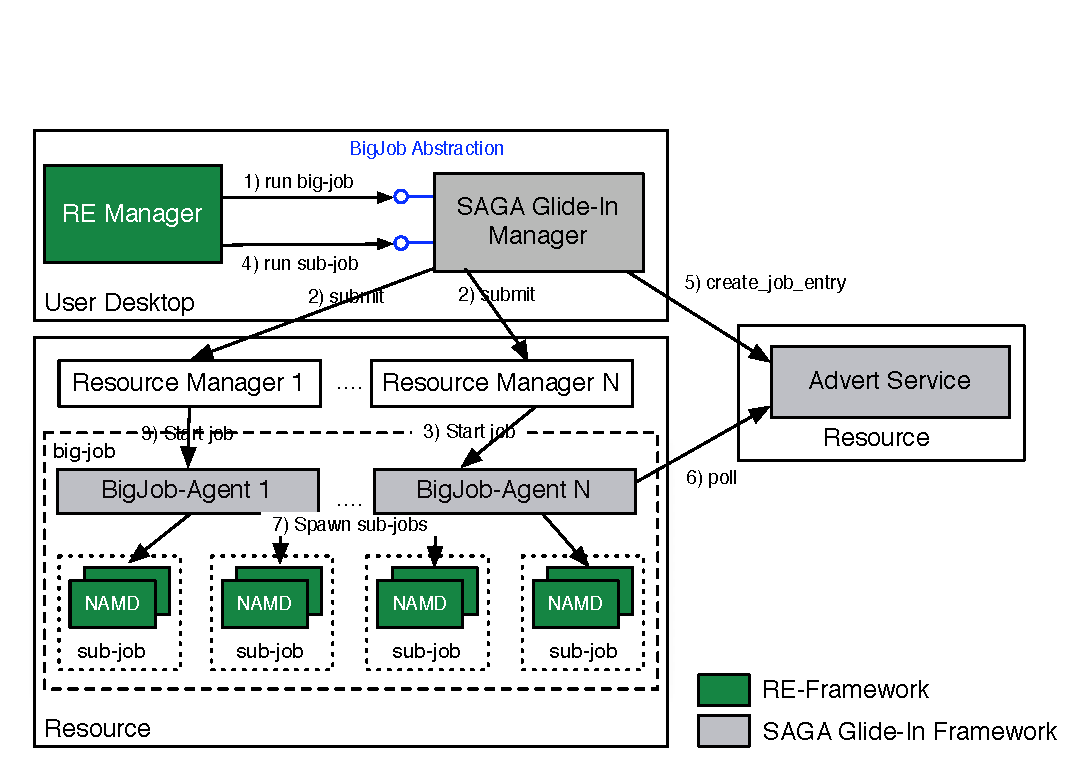
\includegraphics[scale=0.65]{../figures/Bigjob_arch.pdf}
          \caption{ \textbf{The RE Framework:} The framework consists of
 		  the RE-Manager and the SAGA BigJob framework. BigJob is 
		  used to efficiently execute replica sub-jobs. The RE-Manager manages 
		  replica sub-jobs and performs replica exchanges.  }
      \label{fig:bigjob}
\end{figure}

\subsection{SAGA BigJob - A Pilot-job Framework}
\label{sec:BigJob}

% The Simple API for Grid Applications (SAGA)(~\citep{saga_gfd90}) is an
% API that provides the basic functionality required to build
% distributed applications, tools and frameworks so as to be independent
% of the details of the underlying infrastructure. SAGA is an API
% standardization effort within the Open Grid Forum
% (OGF)~\citep{ogf_web}, an international standards development body
% concerned primarily with standards for distributed computing. 

Figure~\ref{fig:bigjob} shows the architecture of the RE Framework --
comprised of the RE-Manager and SAGA BigJob framework. 

SAGA~\citep{saga-url} %\athotanote{2011?}
is an API for the basic functionality required to build distributed
applications, tools and frameworks. SAGA was designed to be
independent of the details of the underlying infrastructure.  We have
previously demonstrated the usage of the SAGA-based pilot-job
framework~\citep{saga_bigjob_condor_cloud} -- called the big-job, to
run RE simulations across multiple, heterogeneous, distributed grid
and cloud infrastructure~\citep{Luckow:2008fp}.

The SAGA BigJob framework consists of three
components: (i) the BigJob-Manager, (ii) the BigJob-Agent and
(iii) the advert service which is a central key/value store used for
communication between the BigJob-Manager and the BigJob-Agent.
The various tasks that are carried out using the SAGA APIs include
file staging, job spawning and conducting the exchange attempts. Here
we use the SAGA BigJob framework to efficiently request and manage
computational resources for multiple replicas and it enables the use of
a range of infrastructure.  For example, we can submit multiple
big-jobs on multiple resources and manage them from one location. 

\alnote{please consistently use hyphen in RE-Manager, BigJob-Manager, ...
Also, SAGA can be removed in front of BigJob Manager.} The RE-Manager requests
a defined number of big-jobs from the BigJob-Manager; for each big-job a
regular batch job is submitted to the resource manager (step 1-3 in
Figure~\ref{fig:bigjob}). When the BigJob becomes active, the BigJob-Manager
can start to process sub-jobs. For each new sub-job an advert entry storing
the description of the sub-job is created by the BigJob-Manager (step 4-5).
The BigJob-Agent periodically polls for new jobs (step 6). If a new job is
found and resources are available, the BigJob-Agent runs the job (step 7). If
not, the job is queued. It is possible that there are more sub-jobs than the
big-job can accommodate. Further, the agent continuously monitors the running
sub-jobs and updates the sub-job states in the advert service. Once a sub-job
finishes running, the compute resources are freed and marked as available.



% \athotanote{check sentence} \alnote{refined. please refer to the
%   advert service as advert service not server (see also
%   figure). Server refers in my opinion to a piece of hardware.}

% The key-value pairs are initially generated by the BigJob-Manager
% and once the big-job becomes active, the BigJob-Agent continuously
% updates the values. The advert service is different from a
% distributed-hash table in that it is a centralised system.  The
% BigJob-Manager submits the big-jobs to the resource manager.
% Sub-job descriptions are store in the advert service. Once a big-job
% becomes active, the BigJob-Agent retrieves the job descriptions from
% the advert server, allocates the required number of nodes and
% launches the sub-jobs on each resource.  The BigJob-Agent
% periodically polls the advert server for new jobs.



\subsection{Replica-Exchange Manager}\label{repexmanager} 

% \jhanote{Abhinav: This subsection should help the reader understand
%   the basic and common elements of the RE Framework -- job submission,
%   role of bigjob-agent, replica-agent, replica-exchange manager etc
%   etc} \athotanote{job submission, bigjob agent are explained in 3a. RE-Manager is explained below. replica-agent is touched upon but a more detailed explanation in section 3b(ii)}
  
%   \jhanote{ABHINAV: DEFINE THE ROLE OF RE-MANAGER HERE.  Possibly BIGJOB
%   AGENT here if not in previous subsection.}  \athotanote{please check if it's ok now}
  
The RE-Manager is the master process which in addition to controlling
the different components -- SAGA BigJob framework, the individual
replicas etc., also defines and implements the coordination/exchange
mechanism employed.  The actual tasks that the RE-Manager performs
depends not only on the RE algorithm employed, but also which exchange
mechanism is being supported.  The RE-Manager supports two different
replica management and exchange mechanisms: centralised and
decentralised. In centralised, the RE-Manager manages all the replicas
and performs the exchanges, whilst in the decentralised case, a {\it
  replica-agent} manages each replica individually as well making and
performing exchange decisions.

% each replica is managed individually by a decisions about how to
% exchange
%The RE-Manager uses the SAGA BigJob-Manager;


% \jhanote{this is an implementation detail. Abhinav: IIUC we restart in
%   both cases -- successful and unsuccessful exchanges. Non? ALso don't
%   toggle between ``replicas'' and ``jobs''!}  

As we will discuss in Section~\ref{sec:re_impl}, the synchronous and
asynchronous RE algorithms were implemented using the centralised
RE-Manager; the decentralised RE-Manager was used to support only the
asynchronous RE algorithm.


\subsubsection{Centralised RE-Manager}

The control flow of a centralised RE coordination mechanism is shown
in Figure~\ref{fig:coordination}(a). A replica can be in one of these
three states: (i) \texttt{new} (submitted but not started), (ii)
\texttt{running} and (iii) \texttt{done}.  Once the big-job(s) is
active and replicas are \texttt{running}, the RE-Manager constantly
queries the BigJob-Manager for the latest replica states.  When the
RE-Manager finds a replica that has finished running, it collects the
energy and temperature of that replica by reading the output
file. Once \emph{all} the replicas have finished running, the
RE-Manager performs the exchanges by swapping temperatures and writing
new configuration files. The new configuration files are staged to the
appropriate location. The RE-Manager then submits the replicas for
restarting, and the BigJob-Manager restarts them. The RE-Manager keeps
count of the successful exchanges, until the required number of
exchanges are done.

We implemented both the synchronous and asynchronous RE using the
centralised version of the framework.  Even though both use the same
framework, the implementation of the asynchronous RE-Manager is
different from the synchronous RE-Manager. The asynchronous RE-Manager
e.\,g.\ is not required to wait for \emph{all} replicas to finish
running before performing \emph{all} exchanges. Whenever the
asynchronous RE-Manager finds a replica that has finished running, it
tries to find a partner to make an exchange. To find a partner, the
RE-Manager goes over the list of all the replicas in the ensemble. If
it finds a replica available it attempts the exchange. If a replica is
not found available, the RE-Manager queries the BigJob-Manager for the
latest replica states and updates its local list. It then loops over
the list to find a replica that has finished running and a partner to
exchange with that replica.  If successful, the replicas are submitted
to be restarted.

\subsubsection{Decentralised RE-Manager and the Replica-Agent}
\begin{figure}%
\centering
\subfigure[Centralised]{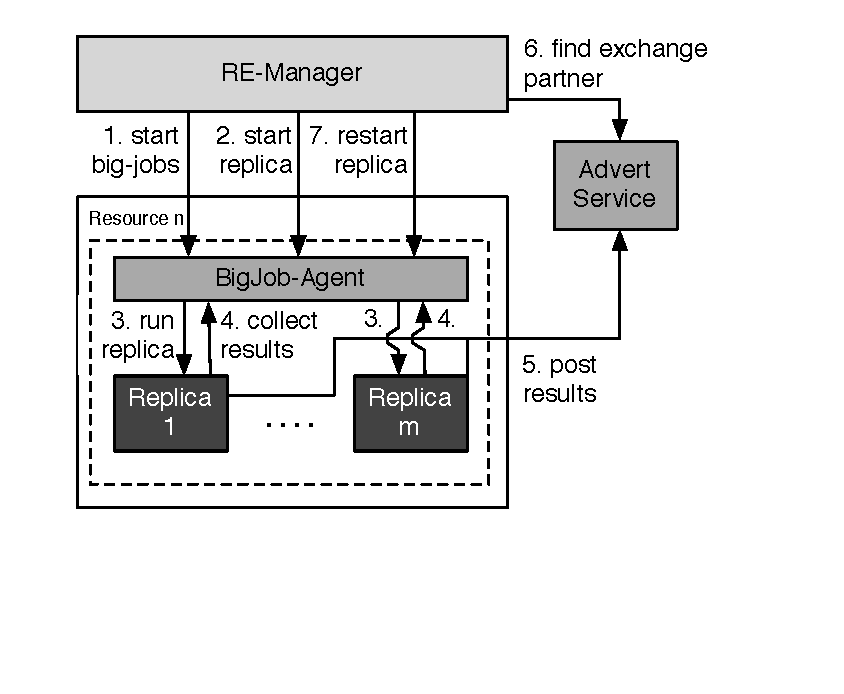
\includegraphics[width=0.49\textwidth]{../figures/central_AL.pdf}}
\subfigure[Decentralised]{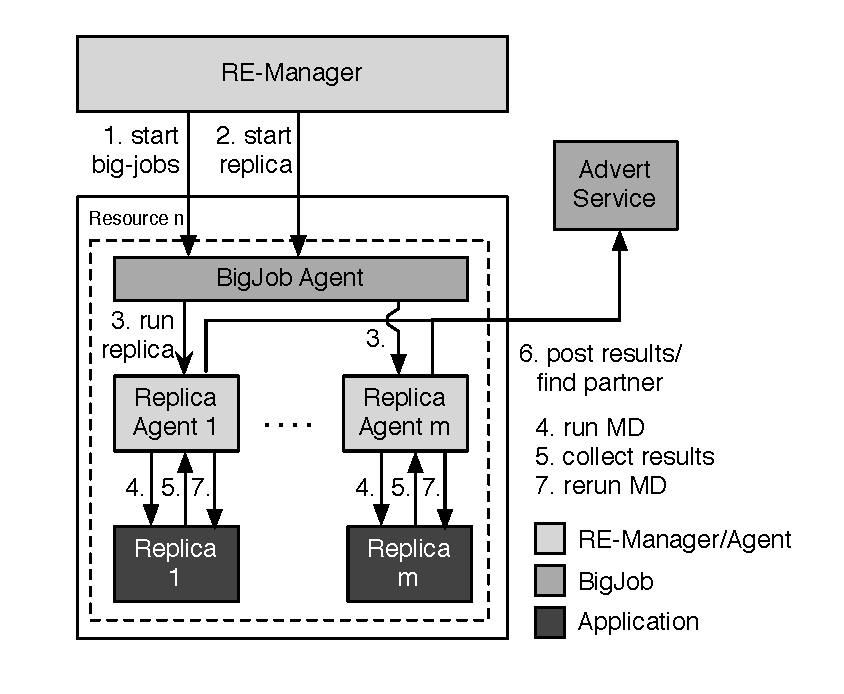
\includegraphics[width=0.49\textwidth]{../figures/decentral_AL.pdf}}\\
\caption{\textbf{Centralised vs. Decentralised RE Coordination:} 
  Centralised coordination style is used by both synchronous RE  and asynchronous (centralised) RE.  In the asynchronous (decentralised) RE --
  the master is only required for initially setting up of all
  replicas. The later coordination is done peer-to-peer via the Advert
  Service.}
\label{fig:coordination}
\end{figure}

% Thus, after the replica-agents are launched, the RE-Manager and the
% SAGA BigJob Manager don't have any responsibilities.
 
Additional states are needed to implement and maintain decentralised
coordination/control.  Thus, the states that a replica can be in the
decentralised RE coordination mechanisms are different to those in
centralised mechanism.  In the centralised implementation, there is no
\texttt{complete} state and in the decentralised implementation there
is no \texttt{new} state. There is no \texttt{new} state in the
decentralised implementation because the replica-agent starts running
only after the processors become available and the replica is started
and put directly in the \texttt{running} state.
 
A replica can be in one of the these four states: in addition to
states (i) \texttt{running}, (ii) \texttt{done}, which were found in
the centralised case, there are also (iii) \texttt{pending} (for an
exchange) and (iv) \texttt{complete} (exchange has been completed)
states.  When a replica reaches a pre-determined state it (the
replica-agent acts as the proxy for the replica) transitions from
\texttt{running} to \texttt{done}. It initiates the search for a
partner, and scans the list of replicas randomly, so as to avoid
contention if multiple replicas have initiated a search for a partner.

If a replica finds a potential exchange partner, it must reverify that both
states are still in the \texttt{done} state. This step is necessary to avoid 
concurrency issues that arise if multiple replicas attempt to exchange with
the same partner. If both replicas are still in
\texttt{done} state, the exchange can proceed and their states are set
to \texttt{pending}.  If the state of any replica has already been
changed (to \texttt{pending}), the  exchange attempt is
aborted.


% \jhanote{This is a way of addressing ``distributed coordination
%   and control.'' Need to mention} \athotanote{check sentence}

% , and waits for its state to
% be set to \texttt{complete} by the other replica (the initiating replica now).
% \jhanote{Is this ``it'' the initiating replica or the ``other
%   replica''?}  \jhanote{Please read the
%   previous sentence carefully: ``... it can restart its replica..''
%   something is wrong!} \athotanote{modified. any better?}


After the exchange is performed (the temperature of both replicas in
the advert server has been changed), their states are set as
\texttt{complete}. Here the state \texttt{complete} is a marker
which tells the replica-agent that the exchange has been made, the
configuration files are in place and to restart the replica.  
The associated replica-agents write new
configuration files with updated temperatures, and restart their
replicas. The replica-agent that initiated the exchange increments the
exchange count. The RE-Manager constantly queries the advert server
for the latest exchange count and when all exchanges have been made,
it stops the experiment.

In the decentralised implementation, in order to conduct the exchanges
the RE-Manager launches multiple replica-agents (in lieu of replicas
directly).  Replica-agents then take control of replica start/re-start
and exchange attempts.  Figure~\ref{fig:coordination}(b) shows the
control-flow in decentralised RE coordination mechanism. The
replica-agents upon launch, run the replicas; a list of nodes that is
used to carry out the MD run is passed to the replica-agent as an
argument at startup.  The replica-agent constantly monitors the
replica, and when the replica finishes, it updates the advert server
with the current state of that replica.  It also reads the temperature
and energy from the output files, and posts the values to the advert
server.  The RE-Manager is primarily responsible for keeping track and
count of the number of exchanges performed; when the desired number of
exchanges are done, the RE-Manager ends the experiment.

%\alnote{paragraph needs attention} 
It should be noted that even in the decentralised implementation, the
advert service is still centralised. Only the replica-management and
exchange coordination are decentralised. We did not observe any
increase in latency with respect to the increasing number of
connections when accessing the advert service.  But the communication
times do vary depending on the physical distribution of the
advert-service. Also, maintaining data consistency is not an issue
because there is only one advert-server.  %\jhanote{What is ``it''?}
Two write actions cannot be carried out simultaneously on a single
value.  It should also be noted that the exchanges are
non-deterministic in nature, first because the replicas available for
exchange are found in a random order and, secondly because, in
principle the Metropolis scheme~\citep{metropolis:1087} is used to
match the replicas.

\section{Executing Multiple RE Algorithms using the RE Framework: Implementation and Performance}
\label{sec:re_impl}
% \alnote{Do we want to present impl. details here?}  \athotanote{i too
%   think that we are explaining how we implemented in section 3(RE
%   Framework). Here we are analyzing our implementation?}
% \jhanote{``Basic characterization of the performance of our implementation''}

In section~\ref{repexfw}, we presented the basic components of the RE
framework and discussed the control flow for the three implementations
of the two algorithm using different exchange coordination mechanisms.
In this section we provide further details of the working of the RE
Framework, as well as a basic characterisation of the performance of
the RE Framework for the three formulations.

% But before that we provide some details of how the RE framework was
% used to implement the different RE formulations.



% as we believe that the asynchronous RE is better suited
% for decentralised implementation.
% We will explain next how the centralised and decentralised replica
% management mechanisms are implemented.


% Further, we analyse the primary components
% that impact the performance of a RE simulation.

For the basic characterisation, the following experimental
configuration is used: (i) Infrastructure: Our experiments are
performed on LONI and the Teragrid shared resource \emph{QueenBee
  (QB)}. A highly scalable, parallel MD code --
NAMD~\citep{Phillips:2005gd}, is used to perform the simulations for
each replica (although, it is important to mention that any other MD
or Monte Carlo code could be used just as simply and effectively with
the RE Framework).  (ii) Replica-Exchange Configuration: The total
number of replicas ($N_R$) in the ensemble is 32 and the total number
of pairwise exchanges ($N_X$) is 128. As the ensemble of replicas are
run concurrently, 16 pairwise exchanges are possible after each
concurrent run. Thus, each replica on average is restarted 7 times.
Each replica is configured to run 500 time-steps and is allocated 16
processors. One big-job of size 512 processors is requested. On
average each 500 time-step run takes $71$ s.  For all implementations,
in the event of a successful exchange, jobs are
restarted~\citep{Luckow:2008fp} with new temperature values.  In the
case of an unsuccessful exchange, jobs are restarted without
exchanging the configuration.  (iii) The physical system that we use
as benchmark is the Hepatitis-C Virus that was examined
in~\cite{Luckow:2008fp}. It is to be noted that in actual biological
science simulations, the number of time-steps between exchanges is
often higher than 500. Thus, the amount of computation performed in
between exchanges is typically higher, thus lowering the cost and
relevance of performing the exchange.

% \jhanote{Can the following be eliminated or moved to someplace later} \athotanote{yes, can be deleted}
% It should be noted that the replicas take longer (91 s) to
% complete their 500 time-steps from a fresh start. But when they are
% restarted, they finish the run slightly faster (68 s).  And the
% total time the ensemble of replicas spend running is $71 \times 8 =
% 568$ s.

Each production run was repeated multiple times  ($\approx$ 10) %during different loads;
%  \alnote{don't understand last part of sentence}  \athotanote{fixed}
and the start time of each run is measured only after the big-job
becomes active.  As we are interested in understanding the scale-up
and scale-out properties of synchronous and asynchronous RE, we do not
consider queue wait-times.  As explained in
section~\ref{sec:repex-approach} (\ref{sec:math-model}), the relative
performance of RE implementations is determined by the waiting time
$T_W$ and the time for conducting the exchange $T_{EX}$. In the
following sections, we analyse the average values for $T_{W}$ and
$T_{EX}$ for each replica pair.  Table~\ref{table:repex_perf}
summarises the results. We will discuss the different RE
implementations in the following sections.  The source-code for
implementing the different RE algorithms using the RE Framework is
available at:
\url{https://svn.cct.lsu.edu/repos/saga-projects/applications/async-re/}.

% Therefore, we start measuring time lapsed only when
% the BigJob agent starts running the replicas/replica-agents because, almost every
% time, the RE-Manager completes submitting them before the
% BigJob becomes active. 
% \jhanote{Is this not just specific to the Synch
%   case? i.e.  for async decentralised case, the replica-agent submits
%   the replicas and not the RE-Manager?!} \athotanote{fixed.}

\begin{table}
    \centering
	\begin{tabular}{|c|c|c|c|}
	\hline
	                        &\textbf{synchronous}  &\textbf{asynchronous (decentralised)} 
	                        &\textbf{asynchronous (centralised)}\\
	\hline
	\hline
	$T_{MD}$       &71\,s &71\,s &71\,s\\
	\hline
	\hline
	$T_{W}$        &2.8\,s &0\,s &0\,s\\
   % \hline
    %\hspace{2mm}$T_{s}$ &2.8\,s &0\,s &0\,s\\ 
    %\hline
%    \hspace{2mm}$T_{r}$ &0 s&0.7\,s &1.1\,s\\
	\hline\hline
	$T_{EX}$        &0.6\,s &7.9\,s &1.9\,s\\
	\hline
	\hspace{6mm}$T_{find}$        &0\,s   &7.1\,s &1.3\,s\\
	\hline
	\hspace{6mm}$T_{file}$       &0.4\,s &0.6\,s &0.4\,s\\
	\hline
    \hspace{6mm}$T_{state}$    &0.2\,s &0.2\,s  &0.2\,s\\
	\hline
	\hline
	$\mathbf{T}$        &\textbf{1003\,s} &\textbf{631\,s}    &\textbf{811\,s}\\
	\hline
    \end{tabular}
    \caption{Average values of terms in Eqn~\ref{eq:totaltime} for the three RE algorithms. $T_{MD}$=time replica takes to complete 500 time-steps; $T_W$=synchronisation time; $T_{EX}$=time to make a pairwise exchange; $T_{find}$=time to find/lock a partner; $T_{file}$=time to write/transfer files; $T_{state}$=time to update states after exchange; $T$=total time-to-completion.} 
	\label{table:repex_perf}
\end{table}

\subsection{Synchronous RE}
\label{subsec:sync}
% The replicas are run by the BigJob agent after the BigJob becomes
% active. The average time the Bigjob agent takes to start one replica
% is 0.3 s.  \alnote{Is this the time agent only? Or does it
%   include the submission time on the master?}  \athotanote{fixed in
%   last lines of the previous section. the time the master takes to
%   submit the replicas is being included in $T_EX$. The time spent at
%   BigJob agent is included in $T_W$. }  \alnote{Don't see any
%   reference to $T_{EX}$ in last section. Later you refer to the
%   resubmission time as $T_{mgmt}$. Also, I don't see this component
%   in the $T_W$ formula below. The reader will not know what to do with
%   the 0.6 sec!}  For a pair of replicas, it is 0.6 s.

% \alnote{Not sure how. But if we have time we should find a way
% to explain better why the post-processing times determines
% $T_W$.} 

In a homogeneous environment the waiting time $T_{W}$ for the
synchronous RE implementation is primarily determined by the fact that
the RE-Manager is only able to process one replica at a time, i.\,e.\
there is generally a delay between the startup of one replica and the
next. Since the post-processing of the replica ensemble takes longer
than the delay between the start-up of first and last replicas, the
post-processing time determines the overall time spent waiting ($T_W$)
for other replicas.  Post-processing involves various state updates as
well as the stage-out of the output file and requires on average
$1.4\,s$ per replica.  Thus $T_{W}$, which is defined for a pair of
replicas, is $2.8\,s$.  For an ensemble of 32 replicas (with 16 pairs)
the delay between the first and last replica transitioning to
\texttt{done} state adds up to $44.8\,s$.
%The waiting time at the BigJob-Agent is subsumed by the synchronisation time, thus the BigJob-Agent is effectively always ready to start replicas, thus, $T_r$ is 0 for synchronous RE.

% \alnote{which is also not really the case since sub-jobs
% are all submitted at once and as we discuss in sec b, the bj-agent 
% processes these sequentially.} \athotanote{this is mentioned above: ``In the synchronous RE implementation replicas are started
% sequentially, i.\,e.\ there is a delay between the startup of the
% first and the last replica. Also, the post-processing of each replica
% run, i.\,e.\ updating the state, marking nodes free, the stage-out of
% the output file, is done sequentially. The longer of the two
% determines the overall time spent waiting ($T_s$) for other replicas.
% In this case the post-processing time is the larger, and on average,
% it takes $1.4\,s$"} 

% As the BigJob agent starts working only after the RE Manager completes
% all exchanges.  



%Thus, $T_W$ is 2.8 s per replica pair.

% That is the time it takes to update the state and
% mark the nodes as free.  Since the whole ensemble of replicas needs to
% complete running, it is sufficient to consider the longer of the time
% to start and the time to mark the end of a replica run. Therefore,
% $T_r$ is included in $T_w$. Since there are 16 pairs in the ensemble,
% for a pair of replicas, $T_w$ is 29.44/16=1.84 s.  

% \alnote{We need to be careful here. If I understand this correctly: stageout of
% file is $T_r$ and stagein $T_{ex}$? Shouldn't we rather consider the stageout
% time above in $T_w$ (since it is part of the delay between the termination of the first
% and last replica)?} \athotanote{i am thinking like this: stageout is done before the exchange and it delays all the replicas becoming available. stagein is done after the exchange. only after the stagein the replicas are submitted to restarting.}

% \alnote{\textbf{included stage-out time into $T_W$ above - just so
%     that you guys can follow my steps (comment and paragraph below can
%     be deleted):} The RE-Manager marks the replicas which finish
%   running as done and retrieves the energies and temperatures by
%   reading the output files. That costs $0.4\,s$ per replica and
%   $0.8\,s$ for a pair. Thus, $T_W = 1.84 + 0.8=2.64$\,s.}


% \alnote{What is the component that is actually spent waiting for the
%   other replicas to complete. The times you mention above are times
%   for actually doing something, but not waiting times!} \athotanote{is
%   it better now?}  
%   \jhanote{in the previous paragraph you write
%   ``seconds''; in the following paragraphs you write {\it sec}. Need
%   consistency!} \athotanote{fixed} \jhanote{Previous paragraph has to be simplified.  Too
%   difficult to understand. REMEMBER: Short simple (ie non compound)
%   sentences}. \athotanote{i think its slightly better now..}

$T_{EX}$ comprises of three sub-components: $T_{find}$, $T_{file}$ and
$T_{state}$. In this scenario $T_{find}$ is $0$\,s due to the fact that there
is a fixed pairing. The updating and stage-out of the configuration
files, is observed to take approximately $0.2$\,s per replica, thus,
$T_{file}$ is $0.4$\,s per replica pair (the transfer of the input files is
done sequentially). 
$T_{state}$ is the time required by the RE-Manager to post a job
description to the advert service. On average $T_{state}$ amounts to
$0.1$\,s per replica, i.\,e.\ $0.2$\,s per replica pair.
Thus, $T_{EX}$ is: $0+0.4+0.2=0.6$\,s. 

%\alnote{moved this from sec b to here (since it also applies heire)}
Although there are $\frac{N_R}{2}$ concurrent pairs, the exchange 
at the RE-Manager is carried out sequentially; thus the effective 
number of concurrently exchanging pairs ($\eta$) is 1.
% \alnote{Not consistent with formula 2.2 where we only define a
%   single $\eta$} \athotanote{fixed in section2}
Substituting the above values in equation~\ref{eq:totaltime}, we get:
% \alnote{TODO: validate numbers with just one decimal position!}
\begin{eqnarray}
  T=  {1 \over p} \times {[ {(71\times {128\over 16}})+ (0.6 + 2.8)\times {128 \over 1}]} = {1 \over p} \times 1003\,s.
  \label{eq:sync}
\end{eqnarray}


% \alnote{Original text: ``$T_{ex}$ includes updating configuration files and transferring them to their
% respective directories; it takes 0.2 s to write and copy a file
% locally.`'' At least in the synchronous version I used there was 
% a remote copy involved. Do we have a number for that?} \athotanote{but this is single machine. local copy right?}
% \jhanote{Abhinav - is the previous sentence correct?
%   ``resubmitting a pair of replicas for restarting'' was too vague!}
% \athotanote{fixed. it may be the case, but we actually explain the
%   actual process after every exchange - that the replicas job
%   descriptions are posted to the advert server, the bigjob agent
%   restarts}
%restart the replicas using the BigJob framework.


% For a pair of replicas involved in the exchange, $T_{ex} =
% 0.2 \times 2=0.4$ s, as file writing and copy is done
% sequentially,
% \jhanote{Should it be $T_{mgmt}$ or $T_{MGMT}$ ? Consistency}
% \athotanote{it should be $T_{mgmt}$, fixed} 
% \alnote{We should be
%   consistent with all subscripts: Why $T_F$, but $T_{ex}$?}
% \athotanote{changed to $T_f$.} \jhanote{Table still needs attention}

% \jhanote{Why is seconds within math mode sometime, and outside math
%   mode at others?}  \athotanote{should we mention somewhere that $p$
%   is one in our experiments and that we dont use metropolis scheme? or
%   can we just leave $p$ as is in the equation?}  \jhanote{For this
%   particular configuration, is this consistent with Data in Section
%   5?}  \athotanote{within error bars, yes.}  \alnote{What about case
%   III: 641+/-2.4 in comparison to 603? But, I guess this doesn't
%   invalidate the model completely}

% \athotanote{yes. i saw this. in the other two cases, substituting
%   $N_X$ in the equation satisfies the all the experiments in section
%   5. but in decentralized, $T_f$ changes with $N_R$. as to why its
%   603 and not closer to 640: i think its something to do the time to
%   find a replica ($T_f$).}

\subsection{Asynchronous (decentralised) RE}

A fundamental difference between the synchronous and asynchronous
formulation of RE is in the synchronisation barrier for the replicas
before exchanges, i.\,e., the former has a barrier, the latter does
not.  As alluded to earlier, we equate fixed replica pairing with
synchronous algorithm, and dynamic pairing with the asynchronous
algorithm. Thus although $T_W = 0$ for asynchronous formulations, this
comes at the cost of a higher $T_{find}$, the time required to
discover a new exchange partner. The lack of a synchronisation barrier
also leads to a more involved implementation to dynamically pair
replicas.

% \alnote{an alternative would be to put the 0.7s into bookkeeping,
%   but not sure whether I want to open that can of worms again...}
% \athotanote{I think we agreed that this is more consistent, because
%   all the bookkeepings are now 0.2 s.  thanks for the refinement. }
\jhanote{Please ``Define'' what this operation is? What part of the equation
?} \athotanote{fixed..?}\alnote{refined}
$T_{find}$ comprises of two components: The pre-exchange management and the actual
search part. As described, in the decentralised implementation of asynchronous
RE algorithm, the replicas are managed and exchanged by replica-agents. The
following pre-exchange steps are necessary: After a replica has completed its
run, the agent updates the replica state at the advert service, which takes
$\approx 0.1$\,s. The replica-agent then retrieves the energy and temperature
from the output file requiring $\approx 2 \times 0.2$\,s. It then posts both
values to the advert service, which takes $\approx 2 \times 0.1$\,s. The total
time for these pre-exchange operations is: $0.1+0.2\times2+0.1\times2=0.7$\,s.
% This $0.7\,s$ is a part of $T_{find}$, which has other components - as explained in the following sentences.  
\jhanote{I find the
  following sentence: out of place. Please place appropriately} \athotanote{removed. i think it is redundant, as we explain this in section 3} %Note that here $T_{find}$ involves pre-exchange management at the replica-agent and not the BigJob-Agent (like the centralised case).

The other component of $T_{find}$ is the actual search time. When searching
for a replica randomly, on average it takes $N_R \over 2$ attempts to find a
replica that is in the \texttt{done} state. However, finding a replica in the
\texttt{done} state is not enough to complete an exchange attempt.
Since there are several concurrent exchange attempts,
contentions and conflicts can arise. Thus, a reverify step must occur before
the exchange is committed. During the re-verification both replica-agents
that are involved in an exchange ensure that there has been state change 
of either of the two replicas involved.  Often, the reverify step leads 
to an aborted exchange attempt. The exact number of necessary attempts is a
random variable, determined by the number of replicas, the
distribution of states and whether the attempt to find a replica is
random or sequential. Empirical observations suggest there are between 2 and 4
find and reverify attempts before an exchange is successful.  
Also, replicas contend with each during this phase: the higher the numbers of replicas,
the higher the contention. That means that $T_{find}$ increases with a higher $N_R$. 
Specifically for the scenario with 32 replicas and random search, $T_{find}$ is 
$2 \times N_R \times 0.1$ (where $0.1$ is the typical time to set/get a value 
to/from the advert service), that is $6.4+0.7=7.1$\,s.
% \alnote{Should we argue with $\frac{N_R}{2}$*4 (in worst case) as
%   previously described or is this too complex?}
% On average the replica-agent must scan
% the list of replicas 2-4 times before it finds a potential partner for
% an exchange (due to conflicts with other attempting replicas).  As a
% consequence of the data-structure and pairing approach used, we find
% that $T_f$ is $0.1\times64=6.4\,s$.

$T_{file}$ includes the process of posting respectively reading the states 
and temperatures to/from the advert service and writing a new configuration 
file: $T_{file}$ is $0.1\times 4 +0.2~=~0.6$\,s. % (And
% even in the other scenario, where the replica in question is not the
% initiator of the exchange, it has to wait for the other replica to set
% its state as complete, so that it can restart).
$T_{state}$ is the time required to update the state in the advert
service, which is $0.2\,s$.  In sum, $T_{EX}$ is $7.1+0.6 +0.2=
7.9\,s$.  It should be noted that $T_{EX}$ is highly dependent on
the actual implementation. While the current implementation is kept
simple on purpose, this value can be improved in a more sophisticated 
implementation.

% \alnote{In the other cases the state must be updated in the
%   advert server as well. Why don't we consider this in the other cases
%   as well?}\athotanote{in the other two cases, the bigjob agent makes
%   the state changes} \alnote{No matter who does the state changes, the
%   time needed should be about the same. Either we put it into the
%   model or we don't. If so, then consistent} \athotanote{we do include
%   the time to update the states. but that is included in $T_W$} 
%   \alnote{Should we just state that there is no central 
%   coordination overhead since the sub-job must not be restarted? And the 
%   time needed to spawn a local process is negligible.} \athotanote{fixed}

% \alnote{The following paragraph can be removed.}
% We also implement a random search of replicas by each replica-agent when the total 
% number of replicas if the ensemble is 128 or more, which reduces contention. 
% It should be noted here that in the centralised implementation of
% asynchronous RE, each query took only 0.01 s. But in
% the decentralised version, each query is shown as 0.1 s. This is due to the fact 
% that each replica-agent stores its replica's data (state, energy, temperature) in 
% a unique directory and changing the directory after each query 
% causes the action to take longer.\alnote{Would it be possible to improve the
% data structure used?}\athotanote{it might be possible..}



% \alnote{Is this the reason why the query takes
%   0.11\,sec instead of 0.01\,sec now? These would be a severe
%   performance degradation.}

% \athotanote{ do we need this para?} In the decentralised implementation, there are many pairs of
% replica-agents negotiating the exchanges concurrently. While this
% causes the time taken per unit exchange to go up, more exchanges occur
% in unit time.

As there are $N_R \over 2$ concurrent exchanges, $\eta$ is 16. Substituting the above
values in equation~\ref{eq:totaltime}, we get:
\begin{eqnarray}
T=  {1 \over p} \times {{(71\times {128\over 16}}) + {(0+7.9)\times {128\over 16}}} = {1 \over p} \times 631~s.
\label{eq:decent}
\end{eqnarray}

% \subsection{Summary}

%\alnote {one could ask why is the config file staged in case I and II then?} 

% \begin{figure}
% \centering
% %\subfigure[Control Flow: Decentralized Replica Exchange]{
% 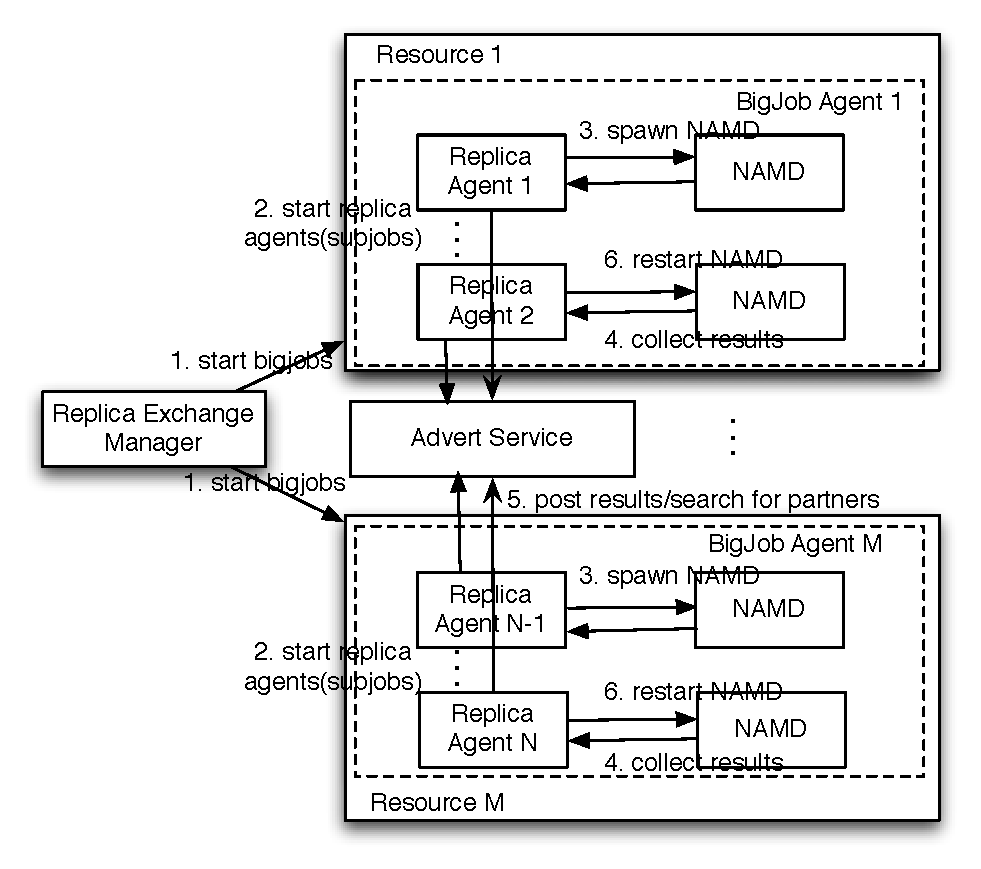
\includegraphics[width=0.9\textwidth]{asyncre.pdf}
% %\label{fig:async:b}
% \caption{\small Decentralized control flow: In the decentralized asynchronous RE, for  each replica there is a replica-agent which individually manages the replica.}
% \label{fig:decent}
% %\vspace{-1em}
% \end{figure}

%\alnote{we should write Case consistently with small or capital letter}
% We have to bear in mind that while Case II and Case III both implement the same asynchronous RE algorithm, they do it differently.
% At first glance it appears to be a question of philosophy, whether to
% let the replicas be managed by a master or to let each replica be
% managed individually.
%There could be implications effecting the performance of the
%algorithm. Where as in Case II, the master has to manage all the
%replicas and since it can only manage one replica at a time, although negligible, it is a cause for concern with large number of replicas. %The effect could be negligible and might now effect the overall performance.
%But the decentralized version (Case III) has no
%such issues as each replica is managed individually. % \jhanote{The distinction between Case 3 and 2 needs to
%  be made more clear. The following is ``implementation detail''. What
%  is the conceptual difference between Case 3 and Case 2?}

\subsection{Asynchronous (centralised) RE}

%As before, the average time the BigJob agent takes to
%start one replica is 0.3 s. For 32 replicas, it is 9.6
%s. Thus, the BigJob agent finishes starting the last replica before the a replica completes its run. 


% ($\eta$ is 1). % \alnote{Not sure
% whether this view helps us here. I am aware of the sequential part
% at the central master, but couldn't that be considered
% quasi-parallel?  Also, the same limitation would apply to the
% synchronous case. An option would be to introduce a $\eta_{MD}$ and
% $\eta_{mgmt}$ in equation~\ref{eq:totaltime}: one for the MD part
% and one for the coordination part.}

% \alnote{I 
%   think this conflicts with the ```deterministic'' approach we
%   discussed yesterday}

% \alnote{``It should be noted that we also implemented a
% special case for an ensemble containing a very large number of
% replicas, where the RE-Manager tries to find a partner randomly. 
% We observed that this only improves the performance when the ensemble
% contains more than 128 replicas.'' Either we should
% state how much this effects $T_f$ or we should not mention it in my opinion. 
% to be discussed} \athotanote{can be deleted}


% If the RE-Manager tries to find a partner for exchange in a linear fashion, 
% it would have to go through 0 to 32 replicas. On average, it would go 
% through 16 replicas to find a partner. $T_f$ is $16\times0.01=0.16\,s$. 
% % \alnote{i.e. per average 16 queries are necessary in
% %   order to find a partner? Why 16?} \athotanote{explained} 
% $T_{ex}$ is the time it takes to
% update the configuration files and copy them locally. That would be
% $({0.2})\times 2=0.4\,s$. $T_{mgmt}$ is the time it takes to
% resubmit the pair of replicas to the advert server, which is
% $0.11\times 2 = 0.22$ s. Therefore, $T_{X}$ is
% $0.16+0.4+0.22=0.78$ s. 

As in the decentralised implementation, the asynchronous centralised
RE formulation does not require synchronisation between {\it all}
replicas in order to transition a replica-pair from \texttt{run\-ning}
to \texttt{done} state and thus, $T_W = 0$ by definition. Using a
centralised RE coordination mechanism, the time to find an exchange
partner ($T_{find}$) can be reduced; however, this comes at a tradeoff
that there is some contention at the master. Also, we observed some
delays at the BigJob-Agent during the startup of the sub-jobs
\jhanote{replicas or sub-jobs? I think sub-jobs!}  \athotanote{fixed} mainly due to the
fact that the BigJob-Agent is single-threaded and thus, is busy
processing other replicas after their termination.  Specifically, the
time-to-submit a replica-pair to the BigJob-Manager, i.\,e.\ two
replica sub-jobs, is on average 1.1\,s for the asynchronous
(centralised) formulation. This is 0.5\,s longer than in cases without
contentions at the BigJob-Agent -- in these cases the submission of
two sub-jobs requires only 0.6\,s.
% post-processing of a sub-job (replica) requires
% 1.1\,s. % \jhanote{Abhinav: Either we multiply by 2 to get pair-wise
% %   value for $T_r$ or we elaborate/explain better} \athotanote{explained} 
% In average every second replica sub-job has a contention with another
% sub-job processed by the BigJob-Agent. Thus, the average time per replica
% pair to restart a replica sub-job is: $T_r = 1.1 / 2 \times 2 = 1.1\,s$.
% For 32 replicas, that would be 35.2 seconds. Therefore, each replica
% pair waits $35.2/16=2.2$ s at BigJob-Agent before being
% restarted. But, we observed that - as the experiment progresses - the
% BigJob-Agent would be processing smaller groups of replicas and
% starting smaller groups of replicas. 
%\jhanote{Abhinav: Andre and I agreed to use 2.2 and not 1.1. Table and values in the Equation need  to be updated to reflect this} \athotanote{but this is the worst  case possible and as the experiment progresses, the bigjob agent  frequently moves between starting and marking jobs as done - instead  of doing 32 in a row. if we make it 2.2 instead of 1.1 there would  not be a difference between synchronous and centralised. and the  equation/model and the data dont support each other.} \alnote{OK,  my original argument fall through after thinking about it. Assuming  a average of waiting for 16 replicas increase $T_r$ even further.   I tried an alternative explanation. Please check!} \alnote{OK,  we settled for a more generell argument talking about sub-job  submission times without speculating how many sub-jobs might  block the processing of another sub-job.}

% On average replica pairs after an exchange actually wait 2.2/2=1.1 s
% to be restarted by the BigJob agent.  \alnote{Shouldn't we use the
%   average number of sub-jobs that a new job has to wait for as an
%   argument?}  Therefore, the value of $T_W$ is the same as $T_r$.
% \alnote{the last sentence can be removed in my opinion.}


% there is some amount of
% waiting involved, which is mainly caused by the single-threaded BigJob
% implementation, which leads to some delays at the agent.
% In particular, a delay arises when new sub-jobs in cases where the
% BigJob agent was busy processing other sub-jobs after their
% termination. In this scenario the post-processing of a sub-job
% requires 1.1\,s about 0.2\,s more than in the synchronous
% case. 
% \alnote{Abhinav please check: in my opinion this is the worst
%   case not the average case. The second replica eg has to wait less.}
% \athotanote{well...}

% In the worst case, the first replica pair that is restarted has to
% wait for the processing of the other remaining 30 replicas: $1.1\,s
% \times 30 = 33\,s$. This corresponds to $T_{r}$ of $1.1\,s$ per
% replica. $T_s$ is 0 in asynchronous RE. Thus, $T_W$ is 1.1 s.\alnote{I
%   still have some issues with that formula i) we don't model anything
%   related to the central master ii) I am not sure whether the per
%   replica view is correct. What is a reasonable $\eta$
%   (resp. $\eta_{MD}$ and $\eta_{mgmt}$) for async RE?}

In contrast to the synchronous case, $T_{EX}$ for the asynchronous
centralised case has a $T_{find}$ component since replica pairs are
dynamically determined and not fixed. $T_{find}$ depends on the overall
number of replicas ($N_R$), which determines the number of records the
RE-Manager has to scan to find an available replica. If random search is used,
the RE-Manager must search through $\frac{N_R}{2}$ replicas on average, before it
finds a partner. Although the search for a replica is random like in the
decentralised implementation, there is no need for reverifying, as due
to centralised control there are no conflicts in replica pairing,
i.e., exchanges are made by the RE-Manager and only one exchange takes
place at a time.  An advert query for a replica state takes
0.01\,s. Note this is a factor of 10 less than the decentralised
implementation. This is because in the centralised case, all the values are located in the same advert directory; where as in the decentralised case, each replica's information is located in a distinct advert directory, so as to enable other replica-agents to find it.  % \alnote{previously,
% we state that multiple connections are not an issue...}
% \athotanote{please comment whether the factor of 10 explanation is
%   necessary/helpful at all? or are we just giving too much
%   information?}
For 32 replicas, the RE-Manager requests on average 16 other replica
states before it finds a partner; thus, $T_{find}$ is in total
$0.01\times16+1.1=1.3\,s$. Both $T_{file}$ and $T_{state}$ are same as
in the synchronous case, i.\,e.\ $T_{EX}$ is thus:
$1.3+0.4+0.2=1.9\,s$.

% \alnote{\textbf{Abhinav: Could you improve the description of this paragraph, please? In particular
% I don't really get the last sentence. Is this the worst or average case? Ok,
% this is the worst case. How do we get the average case?} \athotanote{to do..}
% As previously described, the BigJob agent has an average delay of 0.92\,s 
% for discovering that a sub-job has terminated and for book-keeping, i.\,e. for
% updating the list of free/busy nodes. But in this
% implementation, we also make the BigJob agent retrieve the energy
% and temperature from the output files, which adds 0.2 s per
% replica. In summary it takes 1.12 $\times$ 32 = 35.84 s for 32
% replicas. 
% % \alnote{This somehow assumes that all replica terminate at
% % the same time, right?} \athotanote{as this is the first iteration, 
% % all replicas will end within those 35.84 s of the 1st and last replica. on a homogeneous resource} 
% As soon as the first pair of replicas are marked as done by the
% BigJob agent, the RE-Manager makes the exchange between that pair of replicas 
% - and that pair of replicas would wait 32.8 s ($35.84-1.12\times2-T_X$) 
% before the BigJob agent is able to restart them.} It can be seen from this 
% equation that later pairs of replicas wait a smaller amount of time before 
% they are restarted by the BigJob agent (the BigJob agent alternates between 
% starting all replicas that are new and ending all replicas that are done). 
% On average, a replica waits $T_r$ = 32.8/32=1.02 s to be restarted. 
%   \alnote{I don't understand 
% the notion of pair in this context. Is 32 sec == $T_W$?}\athotanote{is it better now?}\alnote{yes. I think
% we can shorten it and directly break the 32 sec down to $T_W$ for 1 replica: 32.8/32=1 sec.} \athotanote{done}

% \alnote{\textbf{I propose to take the rest of this paragraph out and
%     not go into the details of $T_r$ and $T_w$:} It should be noted
%   that the timelines of the RE-Manager and the BigJob agent run
%   concurrently. Also, the time RE-Manager waits for the next replica
%   to become available, $T_w$ is included in $T_r$. This is because we
%   already included the time each replica waits at the BigJob agent
%   before it is restarted ($T_r$). This would be the same time a
%   replica waits for the next replica to become available. Thus, $T_W$
%   is $1.1\,s$. } \alnote{That is somehow imprecise now! We should only
%   include it in one component.} {\athotanote{this $T_w$ is not
%     $T_W$. it is only part of $T_W$(time waiting for the next replica
%     to become available.  therefore, $T_W$ is still left with
%     $T_r$(time waiting to be restarted at the bigjob agent }
%   \alnote{My point is that the last sentence confuses the reader:
%     either it is $T_f$ or $T_w$.} \athotanote{corrections made.}
%   \athotanote{can be deleted}



% The point we are trying to make is that the BigJob agent might not
% be free while the RE-Manager submits the replicas to be
% restarted. But as the experiment progresses, instead of all the
% replicas in the ensemble running in synchronisation, pairs of
% replicas would start and end together.  By the time the BigJob agent
% finishes processing the last of the replicas that finished running,
% the RE-Manager would have re-submitted 15 pairs of replicas to the
% advert server for restarting by the BigJob agent. In the next couple
% of s the rest of the replicas would have been exchanged and
% submitted to the advert server.

% \alnote{TODO Abhinav: roundup numbers to one decimal place}
% \athotanote{done}

% Although there are $N_R \over 2$ concurrent pairs, the exchange at the
% RE-Manager is carried out sequentially; thus the effective number of
% concurrently exchanging pairs is 1.  

As in the synchronous case the effective number of concurrently
exchanging pairs is 1 due to the fact that exchanges are sequentially
carried out by the RE-Manager.  Substituting the above values in
equation ~\ref{eq:totaltime}, we get:
\begin{eqnarray}
T=  {1 \over p} \times {[ {(71\times {128\over 16}}) + (0 + 1.9)\times {128 \over 1}]} = {1 \over p} \times 811~s.
\label{eq:cent}
\end{eqnarray}

\section{Scale-Up and Scale-Out: Experiments and
  Results}\label{sec:performance}

To evaluate the scaling properties of the different RE
implementations, we conducted several experiments on TG and LONI
resources. We initially increased the number of replicas on a single
machine (``scale-up"); for the asynchronous-centralised
implementations we varied the number of distributed machines used
(``scale-out'') for different replica counts. In this section we
discuss the experiments performed and analyse their results. For both
scale-up and scale-out experiments we find that even though
implementation details are important, the asynchronous RE algorithms
have better scaling properties than the synchronous algorithms.

% Results of these experiments
% establish the advantages of asynchronous formulations for both
% scaling-up and scaling-out.

% \alnote{Should we reference the model used? Not sure which model it is
%   Hepatitis or HIV?}

%
%%%%% FIGURE %%%%%
\begin{figure}
\centering
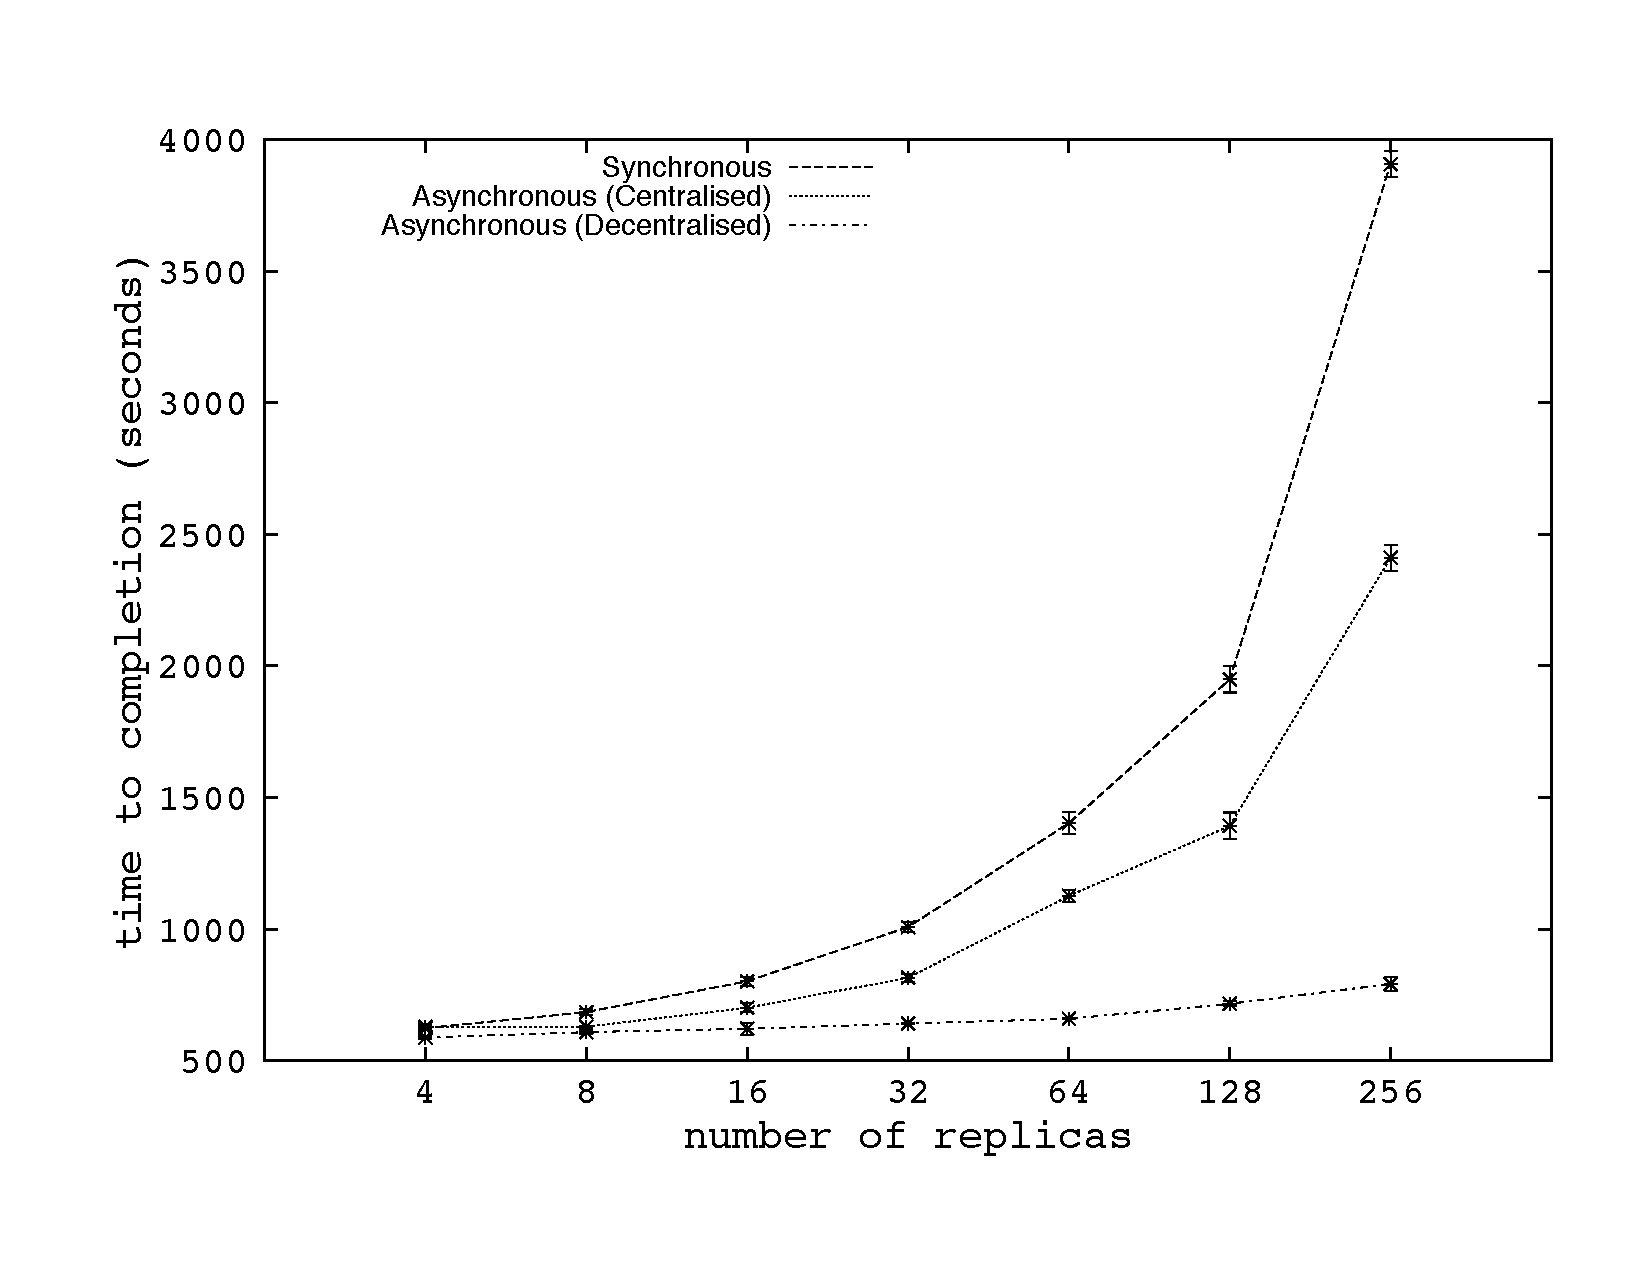
\includegraphics[width=0.8\textwidth]{../data/scale_up.pdf}
\caption{\small \textbf{Scale-Up Performance for 8 to 256 Replicas:}
  The graph shows the runtimes for the different RE implementations.
  The ratio between the number of exchanges and number of replicas is
  kept constant. Each replica is assigned 16 processors and run 500
  time-steps.  The asynchronous decentralised RE implementation shows
  the best scaling behaviour. Both centralised RE versions scale less
  well mainly due to the limitations of the single master, which
  becomes a
  bottleneck.}%\athotanote{there is a graph with log scale in svn, if needed.}
\label{fig:scaleup}
\vspace{-1em}
\end{figure}

% \alnote{The notation of the x- and y-label is kind of confusing. On
%   the y-axis the unit is in parentheses. On the x-axis
%   \#exchanges. Since we keep the ratio between \#replica and
%   \#attempted exchanges constant, do we need both values on the
%   x-axis?}

\subsection{Scale-Up}


{\it Experiments: } To understand the scaling behaviour of the
different RE formulations, we analyse $T$ for replica counts from 4,
8, 16, 32, 64, 128 and 256 making 16, 32, 64, 128, 256, 512 and 1024
exchanges respectively. This fixes the ratio of the number of
exchanges to the number of replicas ($N_X \over N_R$) to 4.  Each
replica is configured to run 500 time-steps before an exchange is
attempted, and is allocated 16 processors. Experiments up to 64
replicas were performed on {\it QueenBee}, while experiments with 128
and 256 replicas were done on \emph{Ranger}; this is because 128
replicas would require 2048 cores and \emph{QueenBee} only allocates a
maximum of 2048 processors per job request. As getting a 2048
processor allocation involves extremely large waiting times in the
queue, \emph{Ranger} was used. We have normalised the data to factor
in the difference in performance of {\it Ranger} and {\it QueenBee}.

% \alnote{this paragraph is in my opinion redundant can be removed}
% The rationale underlying the design of experiments is to understand
% the performance of the different implementations as $N_R$ is
% increased. Given that we understand the performance for 256 replicas,
% we are confident that we can predict the performance of different
% implementations for even larger $N_R$.

% e have seen the results for 256 replicas, we The reasoning behind
% this design of experiments is to understand the behavior of the
% different implementations as we increase $N_R$. The reason we did
% experiments with larger $N_R$ is to ascertain the behavior of the
% different implementations. Now that we have seen the results for 256
% replicas, we are confident that we can predict the performance of
% different implementations for even larger $N_R$.

%\subsubsection{Scale up performance: Results and Analysis}
%\alnote{please double-check that the new abbreviations are used!
%$T_{EX}$}

{\it Results:}   % The ratio of the number
% of exchanges ($N_X$) to the number replicas ($N_R$) is kept constant,
% i.e., the number of generations is a constant for different replica
% counts. 
As a consequence of the ratio of the number of attempted exchanges to
the number of replicas being a constant, the number of times each
replica is restarted to complete all exchanges remains constant; hence
comparison between different cases will reveal differences in the
coordination cost ($T_W$~and~$T_{EX}$). % \alnote{next sentence repeats
% content of previous sentence and can be removed in my opinion} Thus, 
% as $N_R$ increases, the variation in $T$ is due to the coordination component
% -- terms $T_{EX}$ and $T_W$ in Equation~\ref{eq:totaltime}.
The increase,
however, is not uniform across the three implementations: it is largest for
synchronous RE, and the least for asynchronous (decentralised) RE. We analysed
$T$ and the values of its components for 32 replicas in
section~\ref{sec:re_impl}(\ref{subsec:sync}); we use this analysis as the
basis to understand the scale-up behaviour of the three formulations. The
results of the experiments are depicted in Figure~\ref{fig:scaleup}. 
The increase in $T$ as $N_R$ increases is non-linear for synchronous and
asynchronous (centralised) RE and linear for asynchronous (decentralised) RE.

% \alnote{\textbf{Next sentence adds not any value besides filling pages -
% unless you explain what we mean by algorithmic and implementation}}

% We explain
% the reasons for this behaviour - algorithmic and implementation - in the
% following paragraphs.
% \athotanote{added preceding sentences}
 
 
In the synchronous RE algorithm, there is an explicit synchronisation of all
replicas. As seen in Table~\ref{table:repex_perf}, $T_W$ is a major component
of the $T$. As $N_R$ increases, the number of replicas that are required to
synchronised at a given exchange step rises as well; consequently, the
total coordination time at each exchange step increases. The cause for the
increase in $T_W$ is mainly algorithmic and arises due to contention at the
central RE-Manager process. Further, some
implementation details, such as the fact that the current implementation of
the RE-Manager is single-threaded, also effect $T_W$.
%While this is a single threaded implementation, the
%cost of synchronisation ($T_W$) is unavoidable even in a decentralised
%implementation. Thus, $T_W$, which is algorithmic, is the major cause for the
%increase in $T$. 
%\athotanote{added preceding sentence}\alnote{re-arranged and refined.}
Assuming $N_R = 64$ and thus, $N_X = 256$; using Equation~\ref{eq:totaltime},
$T_W$ is can be approximated to $(0.6+2.8) \times 256 = 870.4$\,s. According
to our model $T_W$ for $N_R = 32$ is $485$\,s, which is consistent with the
change in $T$ observed in the experiments depicted in 
Figure~\ref{fig:scaleup}.
% The actual difference observed in $T$ from 32 to 64 replicas is 366 s. % \jhanote{Abhinav: Please provide value of the difference in T here please} %\athotanote{mentioned} 
A similar analysis was performed for different replica and exchange counts and
the values obtained are in agreement with the empirical data in
Figure~\ref{fig:scaleup}.


For asynchronous (decentralised) RE, $T_W$ is 0.
$T_{find}$ has a strong $N_R$ dependence.  The finding operation
involves several queries to the advert service; $T_{find}$ can be
approximated as follows: $2 \times N_R \times 0.1$ (where $0.1$ is the
typical time to set/get a value to/from the advert service).  From
Section~\ref{sec:re_impl}(b) and Equation~\ref{eq:decent}, it can be
derived that for 64 replicas, $T_{find}$ is approximately $0.7$+ $2
\times 64 \times 0.1 =
13.5$\,s. % \alnote{Where do the 0.7 come from? $T_{file}$?}
% \athotanote{fixed}
The difference in the coordination cost ($T_{EX} \times {N_X \over
  {N_R \over 2}}$) between a $N_R$ value of 64 and 32 is 45\,s, which accounts
for the bulk of the increase in overall $T$. % \alnote{if I do the
%   numbers: 32*2*0.1=6.4s and not 45s?}
% \athotanote{corrected
%   explanation}
% The actual difference observed in $T$ from 32 to 64 replicas is 18 s.\jhanote{Abhinav: Please provide value of the
%   difference in T here please again}.\athotanote{done}
%The variation in $T$ for other values of $N_R$ can be accounted for by changing
%values of $T_{find}$.  
The observed performance behaviour can be attributed to both the algorithm, 
i.\,e.\ the used random search method, as well as to specific implementation details, such 
as the usage of the central advert service. 

% \athotanote{added preceding sentence} \alnote{Is this correct? I mean
% how could one implement a better find operation? There must a minimal overhead
% for finding another replica - and I think this overhead also 
% has a $N_R$ dependence}\alnote{refined after discussion during call}

% For 64 replicas, $T_f$ is approximately $1.5 \times 64 \times 0.11 =
% 10.56$ s.  Only $T_f$ changes with the number of replicas.

%  \alnote{Next two sentences: How much does this really impact the
%    decentralised case?  Also, we defined $T_s$ as 0}

In contrast to asynchronous (decentralised) RE, $T_{find}$ in
asynchronous (centralised) RE is only weakly dependent on $N_R$;
however, since the RE-Manager makes the exchanges serially, we still
see an increase in the time-to-completion with increasing
$N_R$. % Using
% Equation~\ref{eq:cent} for 32 replicas as a basis:
For $N_R =$ 64 and $N_X=$ 256, using Equation~\ref{eq:cent} leads to a
new coordination ($T_W + T_{EX}$) time of $(0+1.9) \times 256 =
486.4\,s$, up from $243.2$ for $N_R = 32$. This change accounts for a
large component of the difference in $T$ as $N_R$ goes from 32
replicas to 64 replicas, as shown in Figure~\ref{fig:scaleup}. The
actual difference observed in $T$ from 32 to 64 replicas is 311~s. We
have verified this scale-up model for different number of replicas and
found it to be consistent with the data in the Figure~\ref{fig:scaleup}. 

%In addition to the above, % explicable changes arising from different
% coordination costs,
As $N_R$ increases and as more nodes of a machine are used, we find
that some of them tend to perform differently, thus influencing the
time-to-completion of different replicas; however, these fluctuations
are are small and do not mask the dominant increase with increasing
values of $N_R$ -- which is primarily due to increased synchronisation
times.

% Therefore, as
% $N_R$ increases, the time to synchronise replicas ($T_W$) typically
% increases, increasing $T$.


%\jhanote{What is the implication of this?} \athotanote{fixed}
% When searching serially, we observed that the replica-agent
% finds a partner after looping over the all the replicas between 2 and
% 2.5 times. 
%makes between 1 and 1.5 times $N_R$ calls to find a partner.

\subsection{Scale-Out: Asynchronous RE (Centralised)}
%\alnote{Please reference figures in text.}
{\it Experiments:} In this section, we scale-out to 2 and 4
distributed resources to evaluate the performance of the asynchronous (centralised) RE.  We used the TeraGrid and/or LONI
resources, viz., \emph{QueenBee, Eric, Louie} and \emph{Oliver}. The
experiments were conducted with 8, 16 and 32 replicas that make 32, 64
and 128 exchanges respectively. These exchanges were repeated on 1, 2
and 4 machines while distributing equal number of replicas on each
machine. It is important to note that all experiments were conducted
using four big-jobs, irrespective of the number of machines used
because varying the number of big-jobs, or the ratio of replicas per
big-job effects the overall performance.  Another important point to
note is that only the experimental runs where all the four big-jobs
become active within $30\,s$ of each other on submission to the
resource manager are considered and included in the results. This is
to remove the effect of queue wait time and to get an accurate
assessment of the runtime. Each experiment was repeated 5 times.

\begin{figure}%
\centering
%\subfigure[8 replicas]{
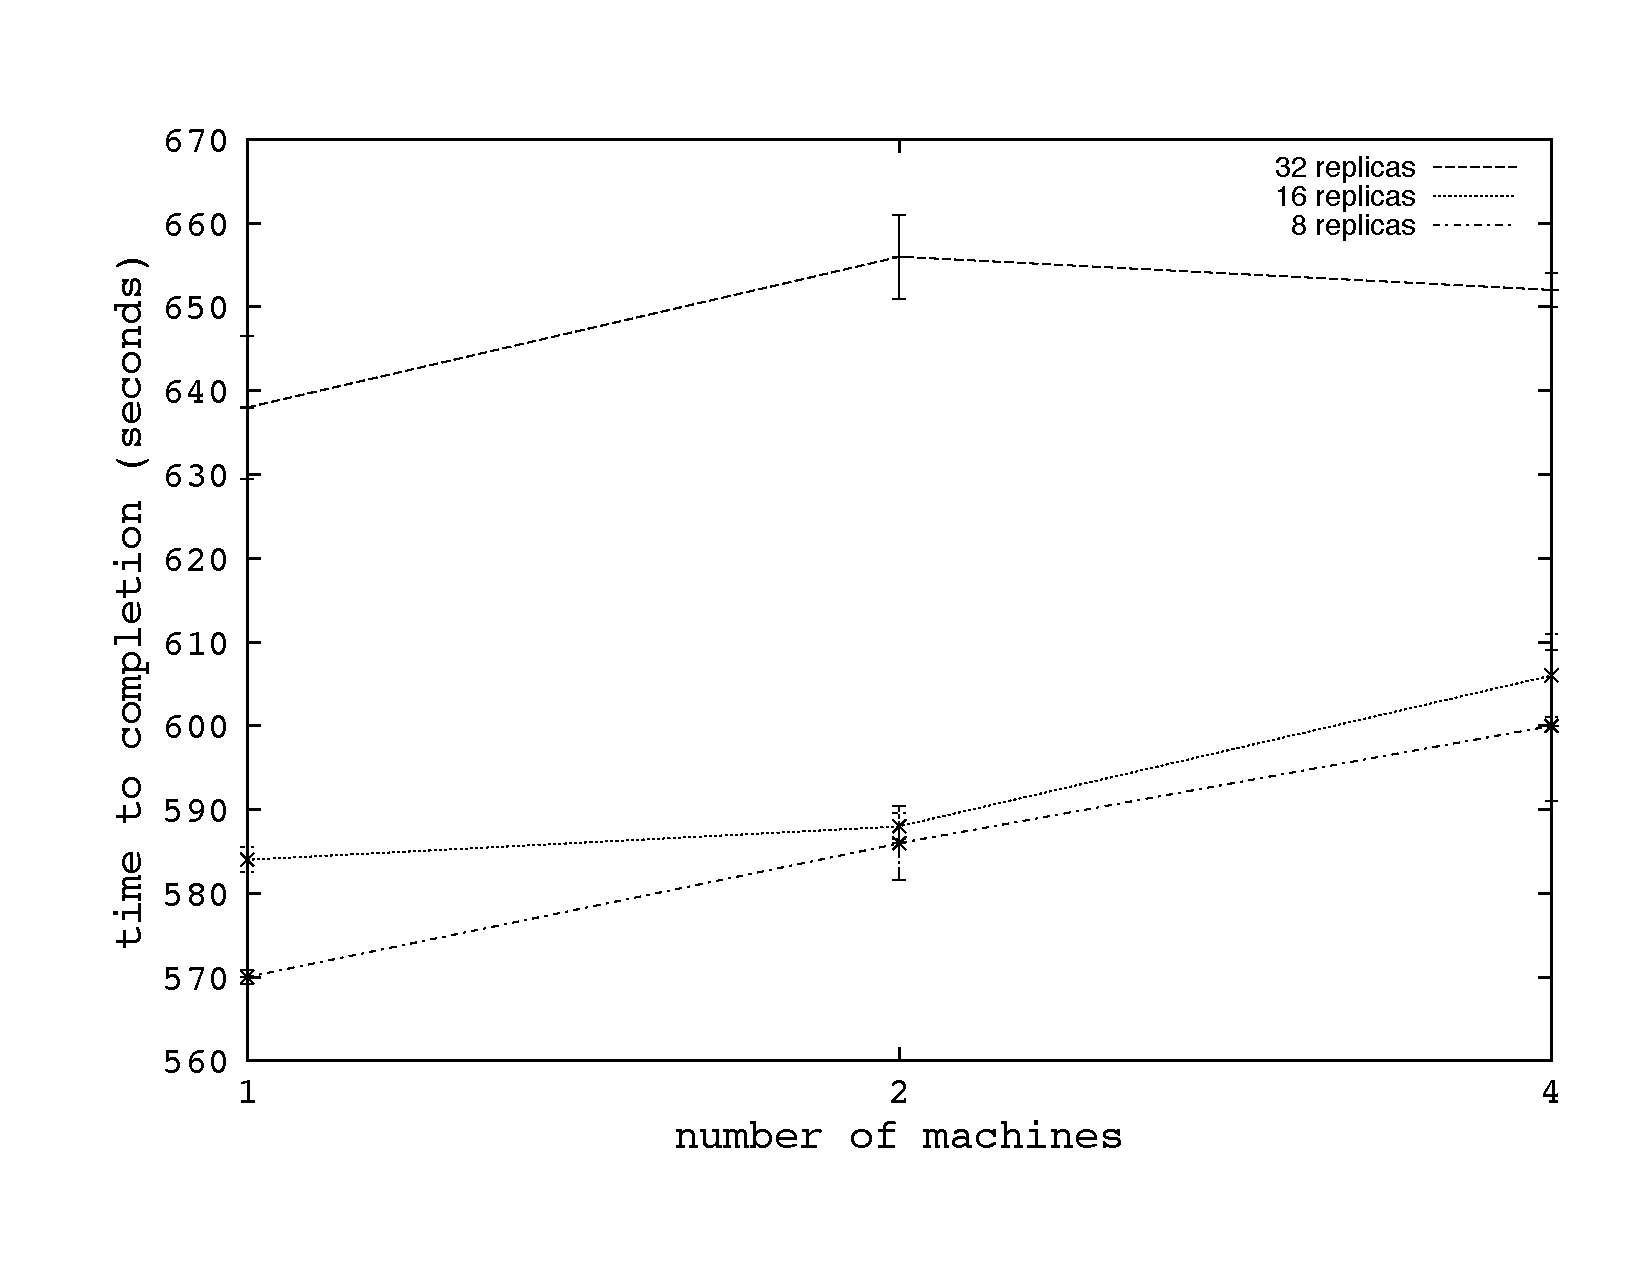
\includegraphics[scale=0.35]{../data/cent_scaleout.pdf}\qquad
%\subfigure[16 replicas]{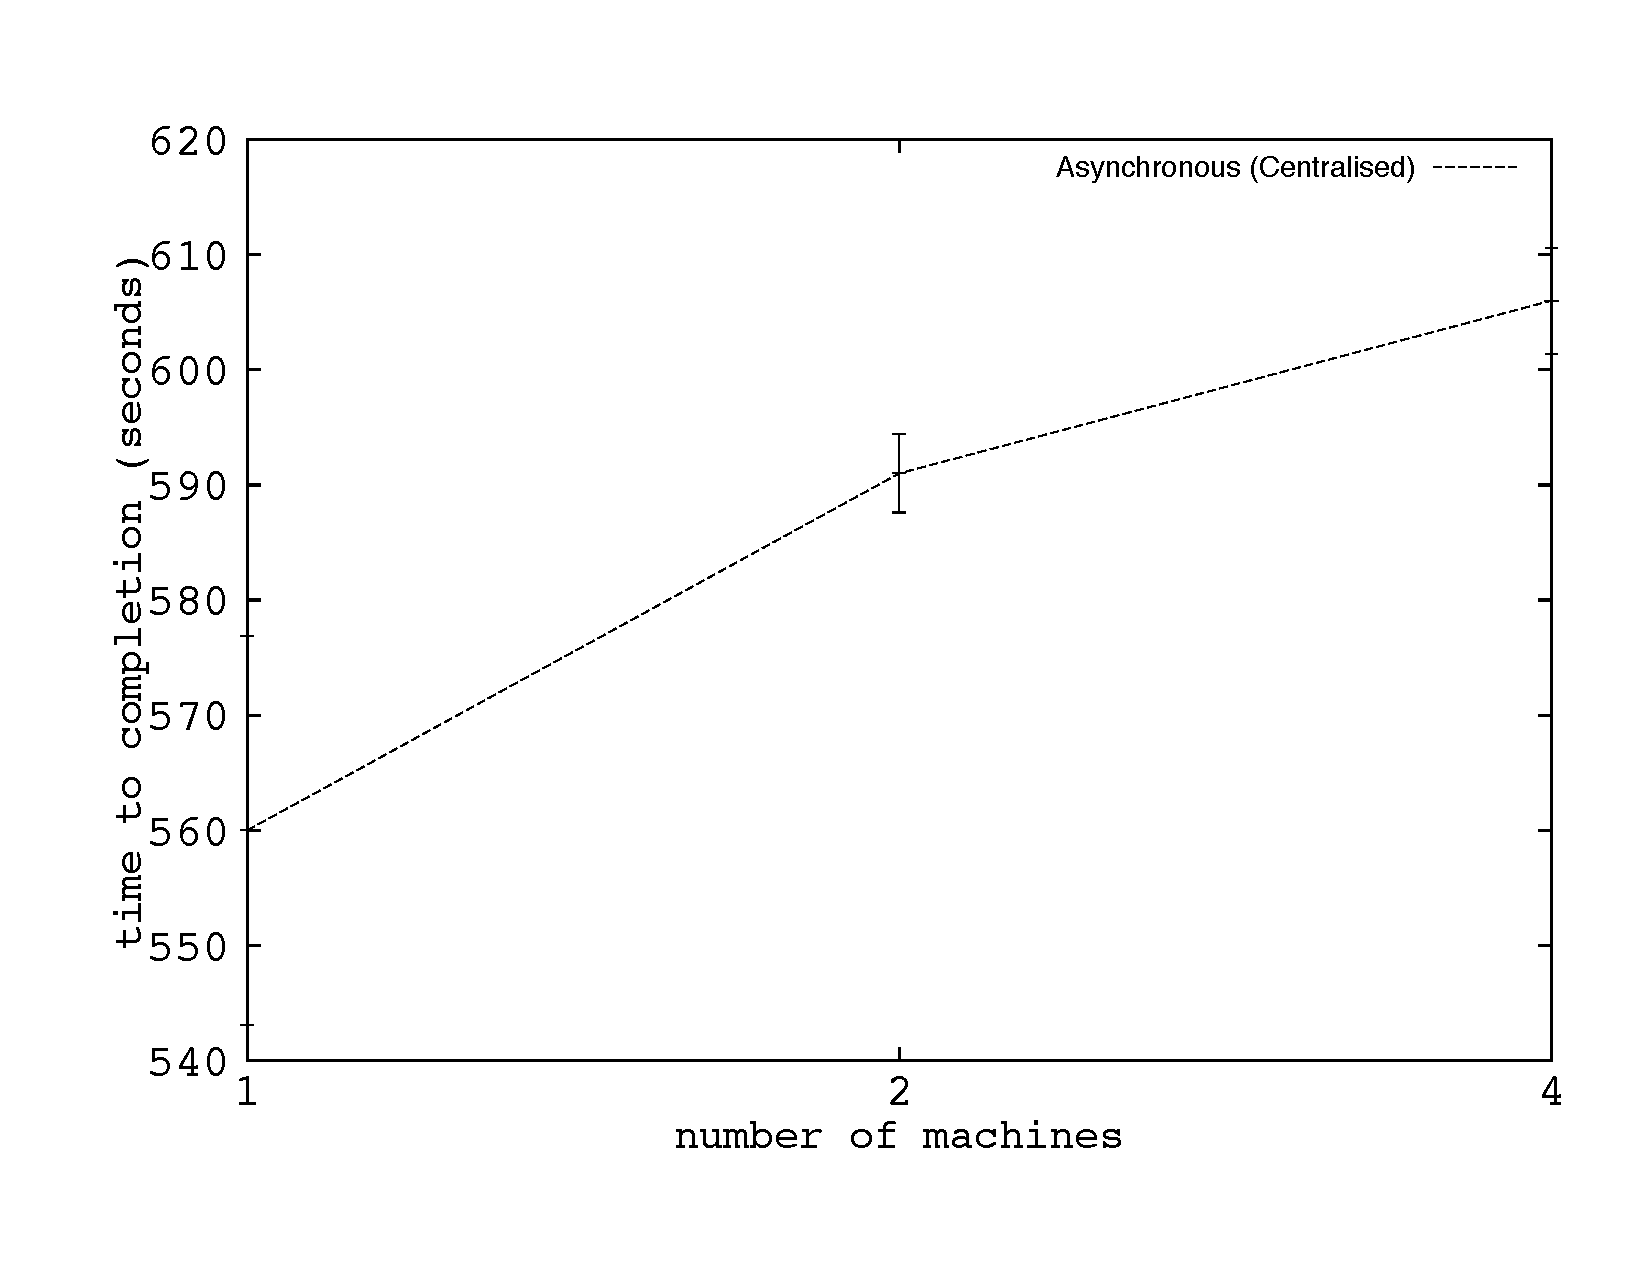
\includegraphics[width=0.47\textwidth]{../data/scaleout_16.pdf}}\\
%\subfigure[32 replicas]{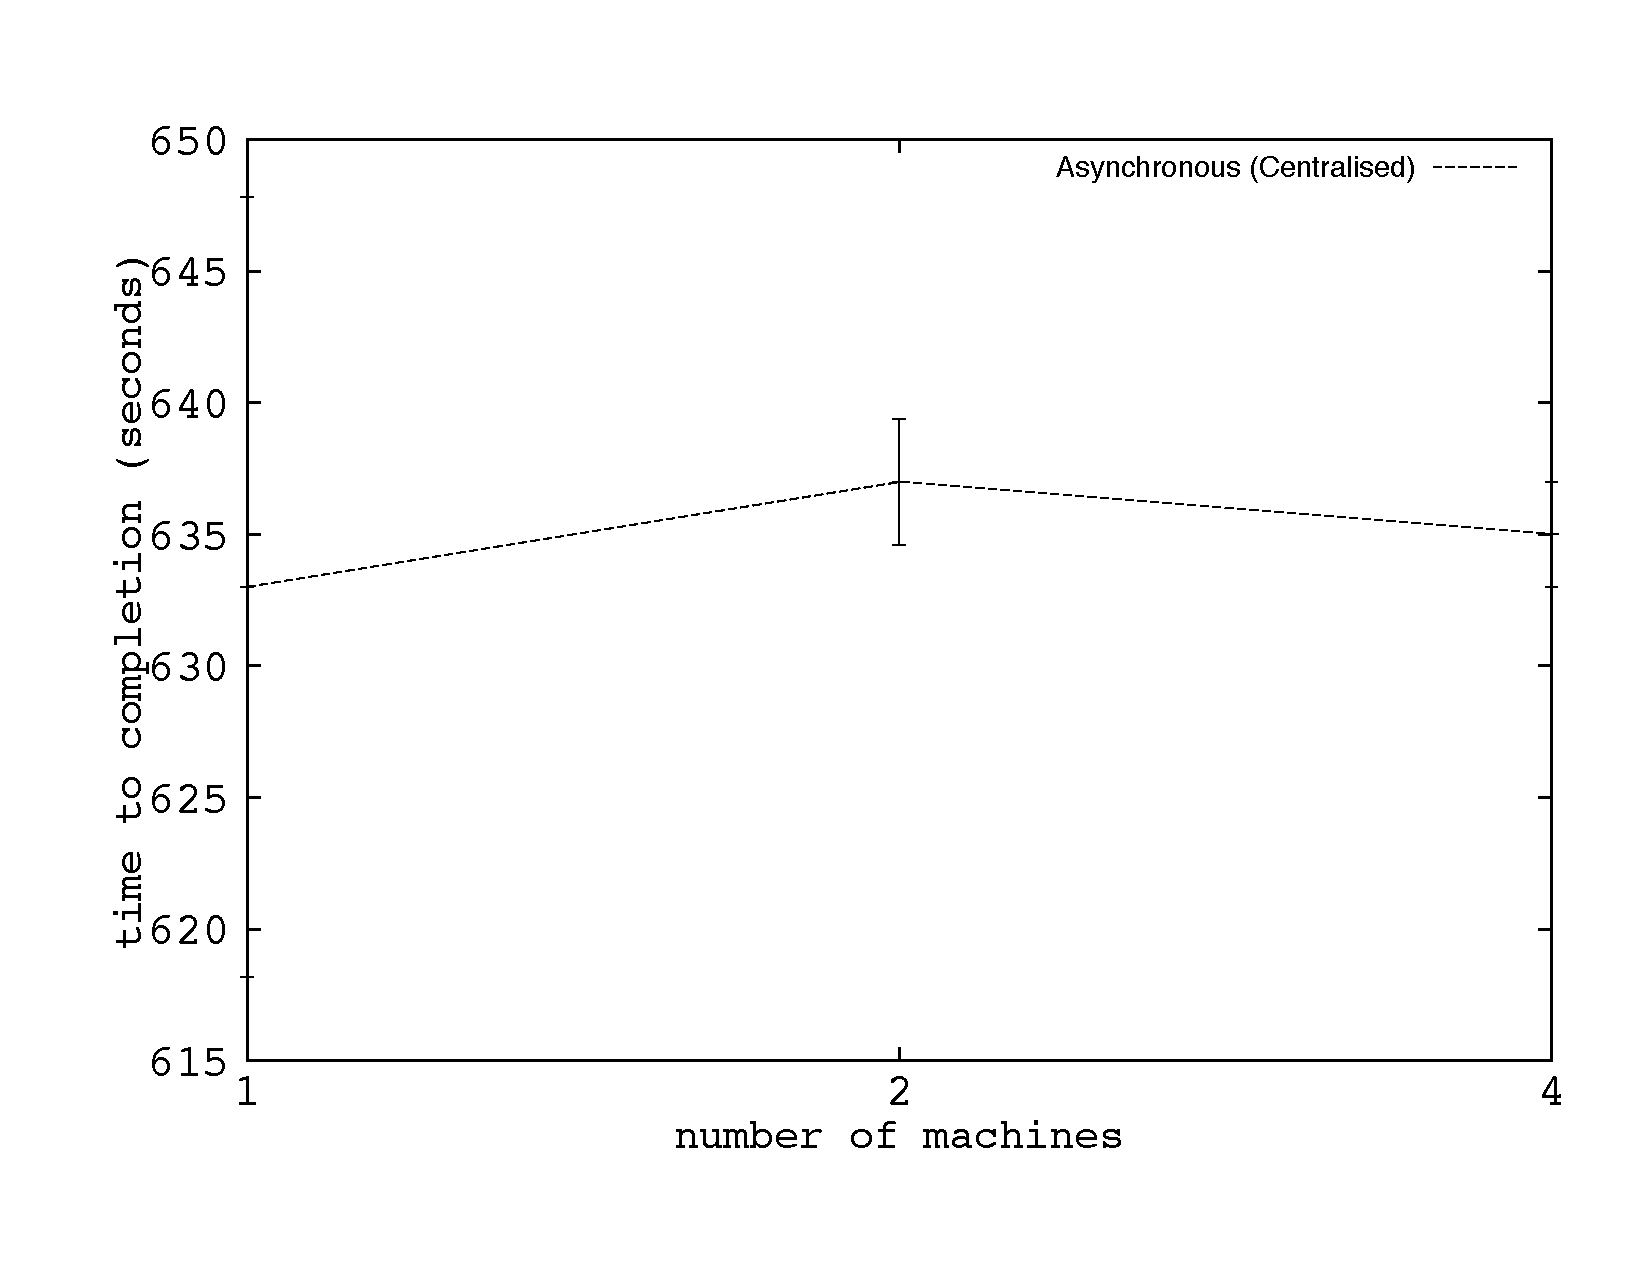
\includegraphics[width=0.47\textwidth]{../data/scaleout_32.pdf}}
\caption{\textbf{Scale-out performance for 8, 16 and 32 replicas, asynchronous (centralised):} 
   The experiments were done on LONI resources and repeated at least 5 times. The error bars denote standard error. As the number of machines increases, the time-to-completion increases in general mainly
  due to higher exchange costs ($T_{EX}$) caused by e.\,g.\  remote file copies.}
\label{fig:scaleout_cent}

\end{figure}

{\it Results:} We analyse the performance of the asynchronous
(centralised) RE using a varying number of distributed
resources (1, 2 and 4 respectively) while keeping the number of
replicas constant. After factoring in the performance advantage due to
the additional big-jobs/BigJob-Agents, the analysis provided
in~\ref{sec:re_impl}(c) can be used to understand the behaviour using
the model developed in section~\ref{sec:repex-approach}.

Even though in a distributed scenario, $T_{MD}$ can be different on
different machines, the resources used in this experiment are mostly
homogeneous in performance, thus, $T_{MD}$ is not effected.  Also,
depending on the physical location and other network related aspects,
$T_{EX}$ can be effected.  Because $T_W$ is 0\,s in asynchronous RE,
the main component that influences $T$ is $T_{EX}$, which is comprised
of $T_{find}$, $T_{file}$ and $T_{state}$. Finding exchange partners
and bookkeeping involves several communications via the advert service
and some local processing. Although the resources are homogenous and
all belong to LONI, they are geographically distributed. This has a
minor impact on the latency observed in the communication with the
advert service: From {\it QueenBee}, {\it Eric} and {\it Oliver} the
creation of an advert entry takes 0.01\,s, from {\it Louie} it
requires 0.02\,s. As the variation in these times is very small, the
impact on $T$ can be neglected. We observed that $T_{file}$ -- i.\,e.\
the time to transfer the configuration file to a replica -- has a
bigger impact on ${T}$.

The results obtained from the scale-out experiments are plotted in
Figure~\ref{fig:scaleout_cent}; note that the scale of y-axis is much
smaller than in Figure~\ref{fig:scaleup}. The variations in $T$ are
small, ranging from 10 to 20 seconds. The fluctuations are all within
the 30 second tolerance imposed by the experimental method. 

For 8 replicas conducting 32 exchanges on 1 machine, $T$ is $570$\,s;
if these replicas are distributed equally over 2 machines, $T$
increases slightly to $586$\,s. In total the observed overhead of
distribution is quite small and essentially acceptable (with at worst
5\,\% of the overall runtime). As explained earlier, the main source
of these overheads are the necessary remote file transfers. Each
remote file transfer takes 0.38\,s while a local transfer requires
only 0.01\,s, i.\,e.\ 0.37\,s less. For the 8 replicas, 32 exchanges
and 2 machines configuration, half of the replicas are located on a
different resource than the RE-Manager, i.\,e.\ the input file must be
transferred to the remote resource in these cases.  On average when 2
machines are used, one of the necessary input files for an exchange
requires a remote copy; for the 8 replica, 32 exchange configuration,
therefore 32 remote transfers are necessary. Thus, the additional
overhead in $T_{file}$ can be approximated to $0.37 \times
32=12\,s$. In Figure~\ref{fig:scaleout_cent}, this accounts for the
difference, to within error bars, between the $T$ values of 1 and 2
machines (for the 8 replica configuration).

As mentioned, we keep the ratio of the number of replicas to the
number of exchanges a constant, thus as the number of replicas
increases the time spent in the exchanges as a fraction of the overall
time becomes less; thus lessening further, any effects of the small
increase due to distributed exchange. This explains why at low replica
counts there is a small (5\%) increase in $T$ as the number of
distributed resources increases from 1 to 4, but effectively there is
no change in $T$ when going from 1 to 4 machines when $N_R$ is 32.

Note that the fluctuations are in the range of 10 to 20\,s. As
mentioned earlier, the big-jobs became active within 30\,s of each
other, thus the fluctuations are within the tolerance of the
experimental design.  Additionally, for the 32 replica configuration,
we see larger fluctuation in $T$ on 1 machine than on 2 and 4
machines.  There are several reasons that can be attributed to the
decrease in the fluctuation in going from 1 to 2 (and 4) machines;
however the dominant reason for the high-fluctuation for 1 machine is
likely to be finite sampling -- recall that experiments were repeated
only 5 times.  We plan to further the number of experimental samples,
and at larger scales to analyse their behaviour accurately.
Nonetheless, from these results, we can say that our RE Framework is
capable of scaling-out without acutely effecting the performance.

% The time-to-completion $T$ increases moderately or remains constant
% with higher number of machines. %it indicates that the scale-out
% %behaviour is quite good. 
% \jhanote{We are inviting trouble with such a qualititative remark.}
% \jhanote{SJ to address earlier why this is to be expected -- based
%   upon Tcoordination/ Tcommunication ratio}

Our model and data from Figure~\ref{fig:scaleout_cent} might only
suggest additional file transfer costs, but in a typical distributed
scenario, with machines on different networks, physical locations,
cost of distributed exchanges and heterogeneity may also play a role
in effecting the performance. We intend to examine these factors in
the future; obviously a comparison with other RE implementations will
also be performed.


\section{Conclusion}
\label{sec:conclusion}

Following on from earlier theoretical explorations,
~\citep{parashar_arepex,DBLP:journals/jcc/GallicchioLP08}, in this
paper, we investigate {\it traditional} and {\it advanced}
replica-exchange algorithms at unprecedented scales.  An important
motivation for this work has been to implement a framework which
supports multiple RE algorithms; it is the aim that the RE
framework use general purpose and standard capabilities available
on production infrastructure, such as, the Teragrid and LONI.
Additionally, our framework uses a flexible pilot-job implementation,
which enables effective resource allocation for multiple replicas.

%that do not enforce a static model of resource usage or availability.
% \alnote{should we be here slightly more concrete and how BJ can help
% here?}

Results shown in figures~\ref{fig:scaleup} and~\ref{fig:scaleout_cent}
indicate that using algorithmic formulations that impose less tight
coordination constraints enables both good scale-up and scale-out
behaviour.  Algorithms based on asynchronous coordination are
typically more difficult to implement than synchronous ones; however,
we find that even with a simple, non-optimised prototype of the
RE Framework, the advantages of asynchronous formulations soon outweigh the synchronous formulations, i.e., as $N_R$ increases the
performance of asynchronous RE beats that of the synchronous RE. 

Our analysis shows that a fundamental trade-off is between the lower
cost of replica synchronisation at the exchange stage that
asynchronous formulations provide, versus the higher cost of
permitting dynamic replica pairing.  In an attempt to investigate an
optimal trade-off between these factors, and to demonstrate the
advantages of asynchronous RE, we implemented a centralised version of
the asynchronous RE with a lower cost of dynamical pairing than in
the decentralised implementation. Our initial results show promising
scale-out behaviour, but more work is required to separate and
understand fundamental algorithmic advantages from implementation
specific issues.



% and scale-out properties on different
% production level infrastructure, 
% Further, we compare the synchronous and asynchronous RE algorithms and
% implementations by modeling and repeating the experiments a reasonable
% number of times, so as to accurately quantify the scientific and
% performance benefits.

%\athotanote{is this right? }
% We are also going to have a wider group of replicas to look at for
% each replica as we are not pairing the replicas.

% Also, we have the usual advantages of using a pilot-job,
% such as reduced queue wait times by not having to submit to the queue
% at every step.  We also provide major advantages when compared to
% Parashar et al.

%  to run the asynchronous RE simulations,
% including the ability to run MPI
% jobs.
% ??We need to evaluate the performance of our models and compare with other models for conducting replica exchange simulations.


%%%%% FIGURE %%%%%
%\begin{figure}
%\centering
%\subfigure[Time to complete 64 exchanges on QB with two 64 core BigJobs and on both QB/Louie jointly with a 64 core BigJob on each machine.]{
%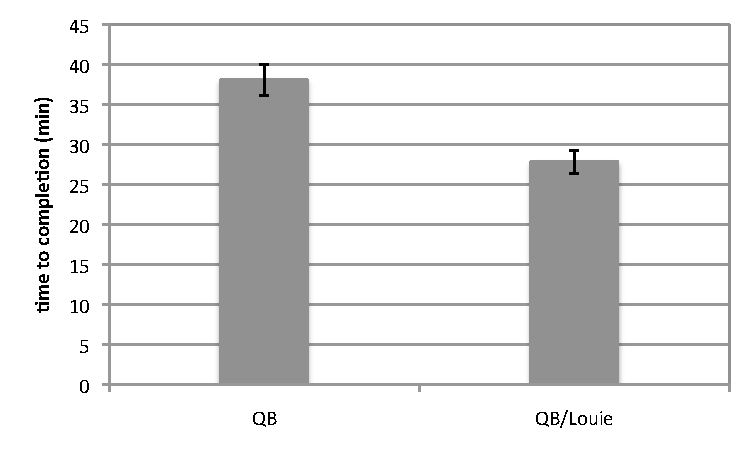
\includegraphics[width=0.40\textwidth]{figures/graph1.pdf}
%\label{fig:subfig3}
%}
%\hspace{0.5cm}
%\subfigure[Time to complete different number of exchanges on QB/Louie with a 64 core BigJob on each machine.]{
%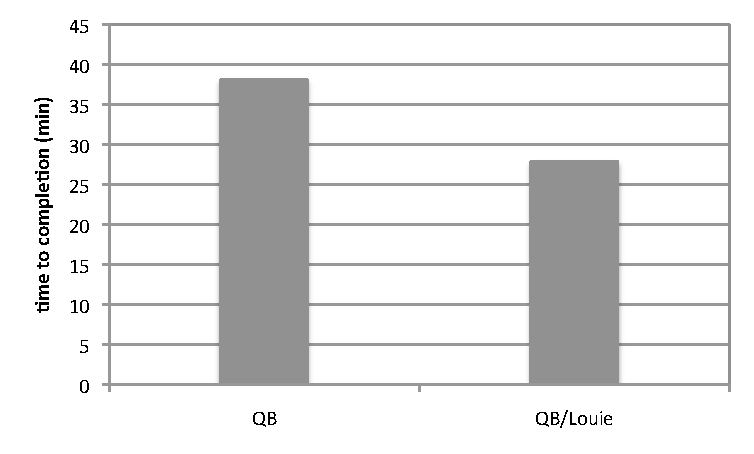
\includegraphics[width=0.40\textwidth]{figures/graph2.pdf}
%\label{fig:subfig4}
%}
%\caption{\small In Figure 2(a), we can see the improvement in performance when run on more than one machine. It is due to the fact that usually the first queued job becomes active before the second on a machine and running jobs on more than one machine solves this problem. In Figure 2(b), we can see consistent performance over prolonged runs, making 32, 64 and 128 exchanges.}
%\label{fig:graphs}
%\vspace{-1em}
%\end{figure}
%%%%% FIGURE %%%%%

%We also propose to measure the frequency with which crosswalks occur with increasing number of replicas and measure the advantages due to a decentralized implementation in the full paper.

%With this asynchronous replica exchange mechanism we can improve the
%number of exchanges per unit time, a key parameter in judging the
%performance of a replica-exchange mechanism. \athotanote{is this
 % right? }  We are also going to have a wider group of replicas to
%look at for each replica as we are not pairing the replicas. Also, we
%have the usual advantages of using a pilot-job, such as reduced queue
%wait times by not having to submit to the queue.  Unfortunately we
%dont have results \jhanote{What results can we present -- any? some?},
%so we will say, (i) we establish the ability to scale-out (distributed
%and exa-scale) across different infrastructure (ii) compare the Async
%versus sync formulation at unprecedented scales \jhanote{At least
%  outline what infrastructure we / you are planning to use?} (iii)
%compare different implementations of the Async version
 

\begin{acknowledgement}
  This work is part of the Cybertools (http://cybertools .loni.org)
  project and primarily funded by NSF/LEQSF (2007-10)-CyberRII-01.
  Important funding for SAGA has been provided by the UK EPSRC grant
  number GR/D0766171/1 (via OMII-UK) and HPCOPS NSF-OCI 0710874. This
  work has also been made possible thanks to computer resources
  provided by TeraGrid TRAC TG-MCB090174 and LONI resources. We thank
  Nayong Kim (LSU) and Tom Bishop (Tulane) for their useful comments
  and suggestions. Computing resources were made possible via TRAC
  award TG-MCB090174.

\end{acknowledgement}

\bibliographystyle{kluwer}
\bibliography{saga,literature}    
\end{document}


% and $T_W=T_w+T_r$, and where
%($T_w$), 

% \begin{eqnarray}
% T = {1\over p} \times [(T_{MD} \times  {N_X \over {N_R \over 2}}) + (T_{X} + T_{W}) \times N_X]
% \label{eq:totaltime}
% \end{eqnarray}

% \alnote{Using ex and EX as subscripts is very
%   confusing!} \jhanote{Why not use T$_X$ in lieu of $T_{EX}$? }

% Equation \ref{eq:totaltime} gives the total time to complete an RE
% experiment. The next equation aims to calculate the time to complete
% particular number of exchanges ($N_z$), where $0 \geq N_z \geq N_X$.

% \begin{eqnarray}
% T_z = {1\over p} \times [(T_{MD} \times  \lceil{N_z \over {N_R \over 2}}\rceil) + (T_{EX} + T_{W}) \times N_z]
% \label{eq:parttime}
% \end{eqnarray}

% Here $\lceil$ $\rceil$ denotes the ceiling function. The reason we put the term ${N_z \over {N_R \over 2}}$ under a ceiling function is because the ensemble of replicas run concurrently and for each concurrent run, $N_R \over 2$ exchanges are possible. Therefore, only the coordination and waiting costs effect the total time. 

% \athotanote{please suggest alternative terms if you find anything
%   confusing}

%It should be noted that only the coordination and waiting costs are divided by $\eta$. The ensemble of replicas are already running concurrently and 


% The RE algorithm involves the concurrent execution of multiple similar
% simulations, the \emph{replicas}.  There is a loose-coupling between
% the replicas in form of periodic exchange attempts between paired
% replicas. The traditional approach to RE is the synchronous model,
% which works well in an ideal scenario with a well defined model of
% resource availability. But with heterogenous systems and fluctuating
% resource availability, the asynchronous RE model could be more
% effectively used to conduct simulations. 
% >>>>>>> .r3441


%Previously, we demonstrated the usage of the SAGA Pilot-Job
%framework~\citep{saga_bigjob_condor_cloud} -- called the BigJob, to run
%RE simulations across multiple, heterogeneous distributed Grid and
%Cloud infrastructures~\citep{Luckow:2008fp}.
%\alnote{maybe we should also intro SAGA at some point} \jhanote{Yes} The Simple API for Grid Applications (SAGA)~\citep{saga_gfd90} is an API standardization effort within the Open Grid Forum (OGF)~\citep{ogf_web}, an international standards development body concerned primarily with standards for distributed computing. The various tasks that are carried out using the SAGA APIs include file staging, job spawning and the conduction of the exchange attempts.
%Further, we introduced several adaptivity modes, e.\,g.\ adaptive
%sampling that are able to react to dynamic changes in resource
%availabilities.

%\alnote{Not sure how many technical we need to provide...}  

%Traditionally, depending
%on the number of processes \texttt{N}, the manager creates \texttt{N/2} pairs
%of replicas.  Before launching a job, the manager ensures that all
%required input files are transferred to the respective resource. For
%this purpose, the SAGA File API and the GridFTP adaptor are used. The
%replica jobs are then submitted to the resource using the SAGA CPR
%API and the MIGOL/GRAM middleware.

%\jhanote{Mention that these are SAGA-based implementations. Something  else would be implemented differently}
%\alnote{Proposed structure: a) math. model b) sync c) async. We should give the reader some orientation in this section.}
% \jhanote{Abhinav: I still note the inconsistent and variable use of
%   algorithms, methods(?) and cases/approaches. I think we should refer
%   to Replica-Exchange as a ``class of algorithms'' or ``algorithm'',
%   and different implementations -- sync versus async} 

% \athotanote{RE class of algorithms - synchronous and asynchronous
%   models within RE class of algorithms; later sync, centralized-async,
%   decent-async implementation. right? or - RE class of algorithms -
%   synchronous and asynchronous implementation of RE class of
%   algorithms; later sync, centralized-async, decent-async
%   implementations. please suggest.}  \jhanote{I would say (i) RE Class
%   of Algorithms, (ii) Sync/Async algorithms too, and then centralized
%   or decentralized implementations of these sync versus async RE
%   algorithm}
%\subsection{Mathematical Model}
%\alnote{I think we should discuss the mathematical model before going
%  into the specifics of sync/async RE.}
%Here we first provide a basic mathematical model for different RE
% models which explains the terms involved. In this section, we aim to
% develop an equation for total time to run any RE simulation. If $t$
% is the average time between successful exchanges, and $p$ is the
% probability of a successful exchange,
%\begin{eqnarray}
%t=  {1 \over p} \times {[T_{MD} + T_{X} + T_{W}]} 
%\label{eq:timebtw}
%\end{eqnarray}
%where $T_{X}$ is the time to carry-out a pairwise exchange, which is
%comprised of (i) finding a partner, (ii) exchanging states including
%file transfer, (iii) book-keeping, and (iv) (re)starting the replica;
%$T_{W}$ is the time spent waiting for all replicas to complete running.
%Therefore, ${T_{X}} = {T_F + T_{ex} + T_{mgmt}}$ 
%and for ${T_{X}}^{async}, T_W = 0$
%The time ($T$) for N$_{X}$ exchanges is therefore $N_{X} \times t$
%If there are $\eta$ independent exchange events occurring
%concurrently, then the time $T$ for N$_x$ exchanges is $T \over \eta$.


% \jhanote{ISNT THE NEXT PARAGRAPH ESSENTIALLY THE SAME AS THE PREVIOUS
%   PARAGRAHGP? WHY DONT YOU REFER TO THE FIGURE AND THE BASIC StePS
%   OUTLINED IN THE FIGURE?}
  
% \begin{figure}[t] \centering
%           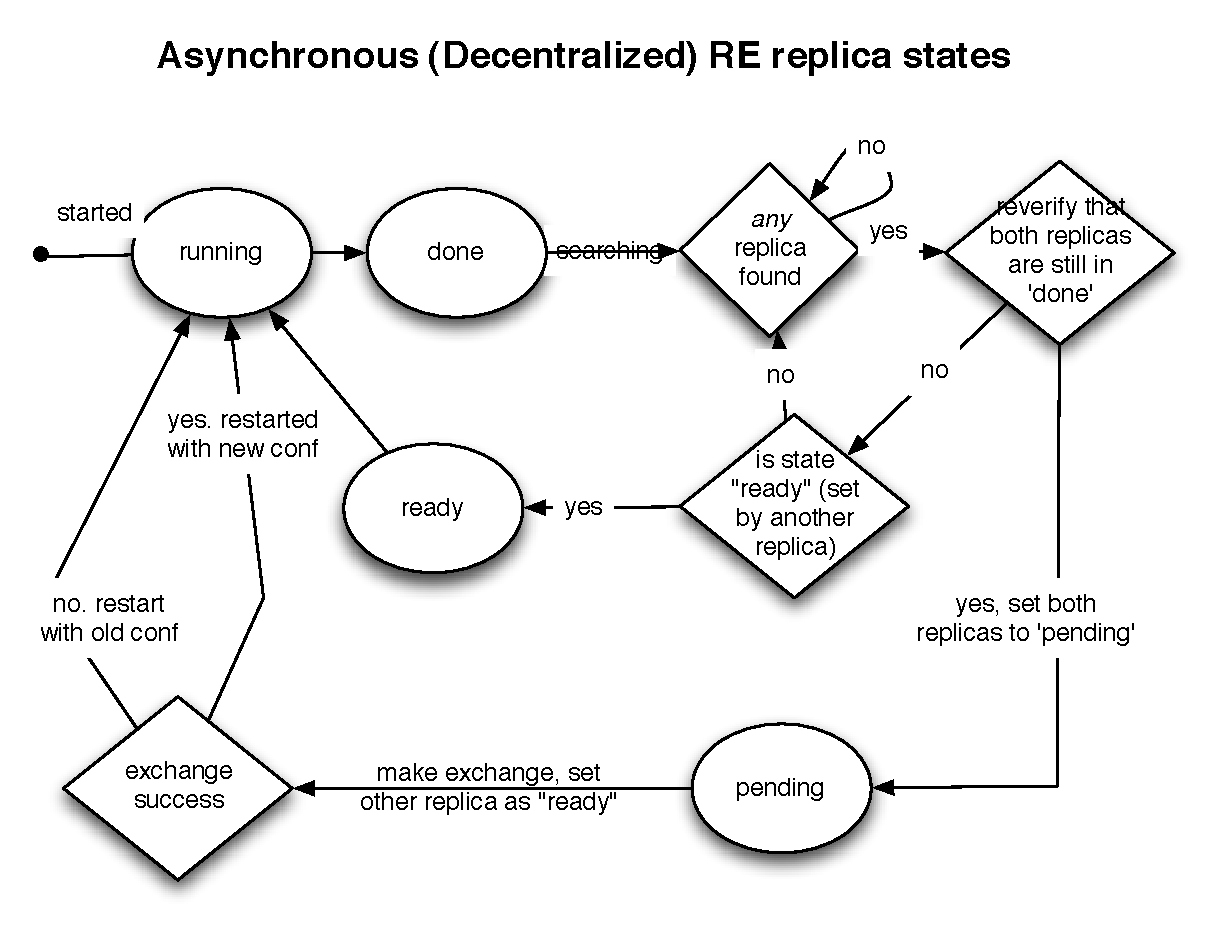
\includegraphics[width=0.82\textwidth]{../figures/decent_state.pdf}
%           \caption{\footnotesize Asynchronous (decentralized) RE
% replica state diagram } \alnote{This chart is not correct yet. There
% can't be state changes on conditional fields} \jhanote{is this a four
% state model or a 3 state model?}
%       \label{fig:state}
% \end{figure}

% As shown in state diagram  (Figure \ref{fig:state}) 
% The replica-agent also goes through the list of replicas randomly to
% try to find an exchange partner.  

% \alnote{In the original state chart we had a ``free'' state. I think
%   this state is needed to ensure the atomicity property of the
%   exchange protocol (2pc style).}
% \jhanote{Would the \texttt{free}
%   state the same as the \texttt{complete} state?}
% \athotanote{i think a replica in \texttt{free} state implies that it
%   is available to make exchanges (meanwhile it also searches or a
%   partner). in the present explanation, that would be \texttt{done}
%   state} 


% \jhanote{Are the four states/description common to all RE cases? If
%   yes, why is it in this paragraph and not in a subsection that is in
%   scope for all three cases? If not, what are the states for the other
%   cases?} \athotanote{not common. added a sentence in the previous section mentioning the states.}

% \athotanote{after an
%   exchange is complete, the state has to be set as complete by the
%   exchange-initiator, so that the other replica-agent can restart its
%   replica} 


%Interestingly, for decentralised implementation, the RE-Manager is functionally similar to the SAGA BigJob-Manager.
%A replica-agent is a wrapper script that manages an individual replica-- starts, facilitates the exchange of that replica, and restarts it.

% And at the least, it is the SAGA BigJob Manager.  At the most,
% launched in place of the replica. The replica-agent implementation
% where the RE-Manager does a lot of work (a centralized
% implementation). But in an implementation where there is a
% \emph{replica-agent} for every replica, the It should be noted that
% synchronous and asynchronous RE are different algorithms and the
% implementation of same algorithm could be centralized and
% decentralized.

%The asynchronous RE algorithm can be implemented using a centralised or decentralised coordination scheme.  
% Synchronous RE is implemented in a centralised fashion. Centralized
% implementation suits synchronous RE because there is a
% synchronisation step at the beginning of each exchange step. But we
% implement asynchronous RE in both centralised and decentralised
% fashions.

% The RE-Manager also creates directories, configuration files and
% stages them to the respective directories.  \alnote{We should focus
%   on the RE part here. The BigJob stuff move to subsec a). This
%   should also remove the redundancy with a)}

%\athotanote{we can remove the sentence about 0.3/10 s, what do you think?}
%\alnote{yes, please remove. Also, I don't understand how 0.3 s can add up to 10 s}
%When the BigJob becomes active, the BigJob agent starts the replica
%agents and the replica-agents in turn start the replicas. It takes 0.3
%s to start a replica-agent (but this is only a one time event and does not influence the overall time to completion by more than 10 s). 

% \alnote{Is it not clear to me: what is $T_{w}$ and what is $T_{r}$? Shouldn't these times
% be lower than in the async-cent. case since we don't have a central coordinator?}


%As in the asynchronous-centralised case the, asynchronous-decentralised implementation does not involve a replica waiting for other replicas to reach a specific state before initiating an exchange. There are other types of holding that contribute to the overall $T$, e.\,g.\ for managing simulation runs, for updating the advert service, etc. Also, queries and updates to the advert service take longer in the decentralised than in the other both case -- mainly due to the higher number of connections and requests. In total, there are three advert updates required: one for updating the state, two for posting the simulation results. Each update requires about $0.1\,s$, i.\,e.\ in sum about $0.5\,s$. Further, about $0.5\,s$ are required for monitoring, restarting replicas as well as processing of output file. Thus, in total $T_{W}$ has a value of $1\,s$ approximately.

 % only includes the time
%spent waiting for the next replica to become available, any time spent
%waiting before the replicas are restarted after an exchange and any
%other miscellaneous costs.

% a pair of replicas are available, and where \jhanote{Is the
%   algorithm similar or identical? If it is not identical, how is it
%   different, or is it just the case that the implementation is
%   different?} \athotanote{is it ok now? i think we are taking the
%   async algorithm as is and implementing it on production
%   infrastructure. ?}
% Let us look at how the ŧō and waiting costs introduced in
% equation \ref{eq:totaltime2} behave. 

% \alnote{This is too general.  We should drop the redundancy of
%   explaining every component and rather analyze the differences.}
% \athotanote{you are right; i am adding a couple of lines here. does
%   it help?} \jhanote{As currently written, $T_W$ has not been
%   defined or ``different components'' discussed, i.e., this
%   paragraph should come after the modelling section}

% But also, an asynchronous RE algorithm has the potential to perform
% better than the traditional RE: (i) when we scale-up the number of
% replicas and (ii) when we scale-out across many machines.
%\jhanote{There is no basis for this sentence at the moment. REMOVE}


% The search for an exchange partner is conducted in a random
% manner when the number of replicas in the ensemble is large, so as to
% avoid having all the replicas starting at the first replica, which
% causes contention and failed exchanges. But for smaller number of
% replicas, a linear search over all the replicas also works. 

% To ensure atomicity of the state transitions, after the initiating
% replica finds an exchange partner, it {\it reverifies} its state,
% i.e., it has not been chosen by another partner in the duration that
% it was finding a partner.  


% \athotanote{i was trying to say the following: replca 1 finds replica
%   2 in done state, but before it locks replica 2, it reverifies both
%   states. (replica 1, while searching could have been set to pending
%   by replica x) If states are still done, the replicas are locked and
%   exchange is made. I made some changes in the explanation. please see
%   if its easier to understand now.}

% \jhanote{I don't understand how its state is
%   set to complete and then to restart the replica} \athotanote{is it
%   better now?}. 
% \jhanote{Do you mean
%   replica-agent?} \athotanote{yes, fixed.}

% At the point where the first replica reverifies the states, if one of
% the replicas' states have changed: (i) if it is the second replica,
% the replica-agent tries to find a new replica; (ii) if it is the first
% replica itself, that would mean another replica has set the replica as
% \texttt{pending}. 

% \subsubsection*{This paragraph to be removed on discussion}

% , it re-verifies the
% states of both itself and the other replica and if both are still
% available, 
% exchanges their temperature values on the advert server.  

% \jhanote{I though the RE-Manager did the following} \athotanote{the
%   replica-agent increments the count, the RE-Manager gets the count
%   from the advert server. Please look at the above para and tell me it
%   makes sense}\jhanote{OK. thanks}

% \jhanote{I don't understand any of the stuff below. State changes have
%   to be atomic!?: If the state of any of the replicas negotiating the
%   exchange changes at the time of re-verifying the replica pair's
%   states, that would mean that one or both of the replicas' is now in
%   the process of making an exchange with a different replica. In that
%   case one or both of the replica-agents will wait till their state is
%   set as "Ready" and start their next run. If one of the replicas is
%   still available, it tries to find a new partner for exchange.}
% \jhanote{Lets talk about this. I
%   don't think another replica should be allowed to change the state
%   of the ``initiating'' replica whilst the ``initiating'' replica
%   is out looking for a partner}

% The search for an exchange partner is conducted in a random manner so
% as to avoid having all the replicas starting at the first replica,
% which causes contention and failed exchanges. If it finds another
% replica available, it re-verifies the states of both itself and the
% other replica and if it finds both still available, marks their states
% as "Pending". Let the replica initiating the exchange be $R_a$ and the
% other replica be $R_b$.  The replica $R_a$ which initiates the
% exchange is the replica in-charge of the exchange. $R_a$ then
% exchanges their temperature values on the advert server.  \alnote{We
%   should detail the exchange protocol. How do we ensure that the
%   exchange is atomic? figure?}  It then modifies its configuration
% files locally, sets its state as running and runs the replica. On the
% other hand, the $R_b$'s state is set as "Ready" by $R_a$ and that
% makes the $R_b$'s replica-agent to retrieve its own temperature
% (modified by the $R_a$) from the advert server, modify its
% configuration file locally and run the replica. \alnote{Why does it
%   need to modify its own config if it uses its own temperature?}
% \athotanote{fixed} This removes the need to stage the configuration
% files to different machines. This is possible because there is a
% replica-agent for each replica locally. Where as earlier, the
% RE-Manager and the replica might be located on different machines.  If
% the state of any of the replicas negotiating the exchange changes at
% the time of re-verifying the replica pair's states, that would mean
% that one or both of the replicas' is now in the process of making an
% exchange with a different replica. In that case one or both of the
% replica-agents will wait till their state is set as "Ready" and start
% their next run. If one of the replicas is still available, it tries to
% find a new partner for exchange.  \alnote{How often is the process
%   repeated until the replica is started with the old temperature?}
% \athotanote{fixed}The replica-agent that initiated the exchange
% increments the exchange count by one.  If an exchange fails due to
% contention, the replica-agent tries to find a new partner. If an
% exchange is deemed unsuccessful after comparison of energies or
% temperatures, the replicas are restarted with their old
% configurations.

% \jhanote{Do we have a pending state? Accoridng to Abhinav there is
%   only a two-state model -- run and done?!} 
% \athotanote{should i keep the state diagram? do you suggest any
%   corrections to the state diagram? i also think that instead of
%   having the current control flows, we should have figures showing how
%   the exchanges are made or instead hae state diagrams. the control
%   flows right now show a lot of stuff already shown in the bigjob
%   architecture figure. }
  
%\section{Implementation of Synchronous and Asynchronous RE}
%\section{RE Framework: Implementation and Performance}

%Therefore the value of $T_W$ $0.7\,s$.

% \alnote{\textbf{Old Paragraph - please check whether I put the important points into
% the paragraph above. Also check my comments in original paragraph.} \athotanote{can be removed}
% \alnote{Initial costs are not really part of our model? Do we 
% need to consider all of them?: 
% The replica-agent initially creates the output and error files, reads the configuration, 
% opens a connection to the advert server, sets the state to running and starts the
% replica. The replica is restarted after every exchange. Therefore, $T_r$, which is 
% recurring is 0.3 seconds.} \alnote{Abhinav: not sure whether I understood everything correct: $T_r$ does not
% include any advert update, or does it?} \alnote{Why does it take longer than in case I/II? 
% \textbf{TODO Abhinav:} separate $T_{mgmt}$ out of $T_r$} \athotanote{done} \alnote{We took
% about 1\,s out of $T_{w/r}$, but only add 0.1\,sec to $T_X$.}
% \athotanote{we are now considering some actions as happening only at
% the start}

% \alnote{How do you get 1.3 sec? The starting of the replica-agent
%   must not be repeated after every exchange, correct?}
% \athotanote{fixed. is it ok now?}

% \alnote{A advert modification took in the previous
% cases 0.01\,sec? What is different here?}.\athotanote{yes, the number of 
%connections to the advert server effects the performance}

% \alnote{Yesterday, it scanned through 15 replicas; in the
%   decent case it scans 16 replica; now it scans 64 replicas. Why is
%   that?} \athotanote{discussed in call.} \alnote{ ok, we still need to
%   explain why we need 4x more attempts than in the async-cent case.}
% \athotanote{done}
% \alnote{Why 15?
%   Previously, it has been 16.} \athotanote{random queries}
% \alnote{Even if it is random, why should the average \# be different
%   in this case compared to the other case?} \athotanote{hmm.. i am not
%   sure. 15 is the average i got after looking at the outputs} 


% This is because, every time the replica-agent finds an
% exchange partner in $N_R/2$ steps, we observe that this needs to be
% repeated 2-4 times as the exchange does not proceed due to conflict
% with another replica.
% Each query requires $0.1\,s$,


% $T_{EX}$ is primarily determined by $T_{find}$, i.\,e.\ the time necessary
% to lock an exchange partner.  

%
%%%%% FIGURE %%%%%
%\begin{figure}%
%\centering
%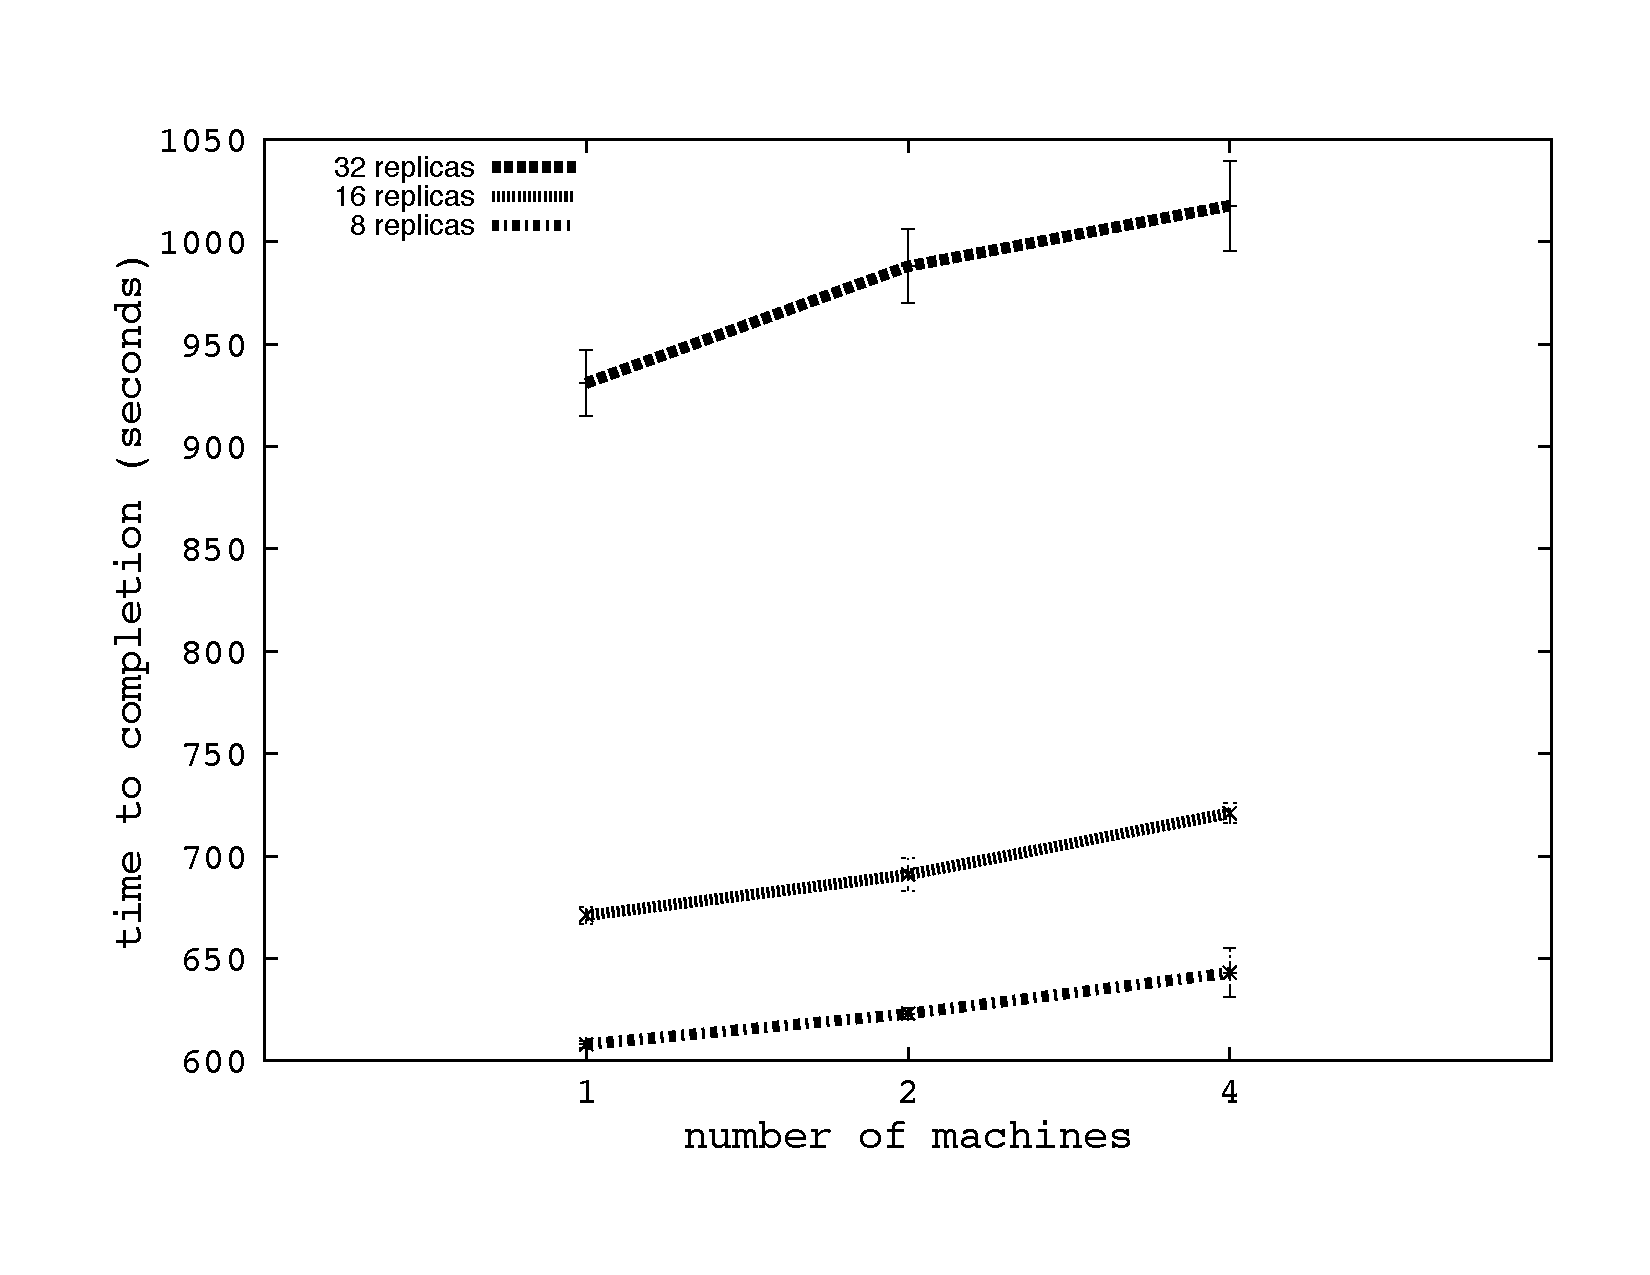
\includegraphics[scale=0.35]{../data/sync_scaleout.pdf}\qquad
%\caption{\textbf{Scale-out performance for 8, 16 and 32 replicas, synchronous:} The experiments were done on LONI resources and repeated at least 5 times. The error bars denote standard error. As the number of machines increases, the time-to-completion increases in general mainly  due to higher exchange costs ($T_{EX}$) caused by e.\,g.\  remote file copies and additional synchronisation costs.}
%\label{fig:scaleout_sync}
%\end{figure}

%\subsubsection{Scale out - Synchronous}
%\alnote{Please use our model from sec 2}
%\alnote{Also, the text does not describe the behaviour with different no. of replicas. Maybe we should merge fig 4-6 into one figure using e.g. 32 replicas.}
%{\it Results:} The results are shown in the graph~\ref{fig:scaleout_sync}. 
%We see that as we go from 1 to 2 and 4 machines, the time to completion 
%increases. The difference in performance that we see as we go from 1 to 2 
%and 4 machines could be caused by: (a) increased synchronisation costs, 
%(b) additional time taken for remote file staging, and (c) higher communication 
%costs to contact the advert server. But the machines we used are similar 
%in nature and the NAMD runtimes are almost close to each other. But still, 
%the NAMD runtimes are not constant and vary slightly from one to another. 
%We do not observe any difference in the 
%communication times with the advert server. Therefore, the factors
%effecting the $T$ is the additional time to stage the configuration 
%files and the slight overhead added to the synchronisation cost.
%
%\alnote{Didn't we decide to abbrev. seconds with s?}
%To copy the configuration file locally it takes 0.009 seconds and to a remote machine it takes 0.379 seconds, approximately. The difference in time is 0.37 seconds. In the graph~\ref{fig:scaleout_sync}, going in the 8 replica case, going from 1 machine to 2 machines, the $T$ changes from 608 to 623 seconds. In the 2 machine case, the RE Manager would have to stage 4 configuration files remotely every exchange step. That would be $4 \times 8 = 32$ times in the whole simulation. That is an additional $32 \times 0.37 = 12$ seconds. And, 608+12= 620 seconds. This holds for 16 and 32 replica cases. 
%
%\begin{figure}%
%\centering
%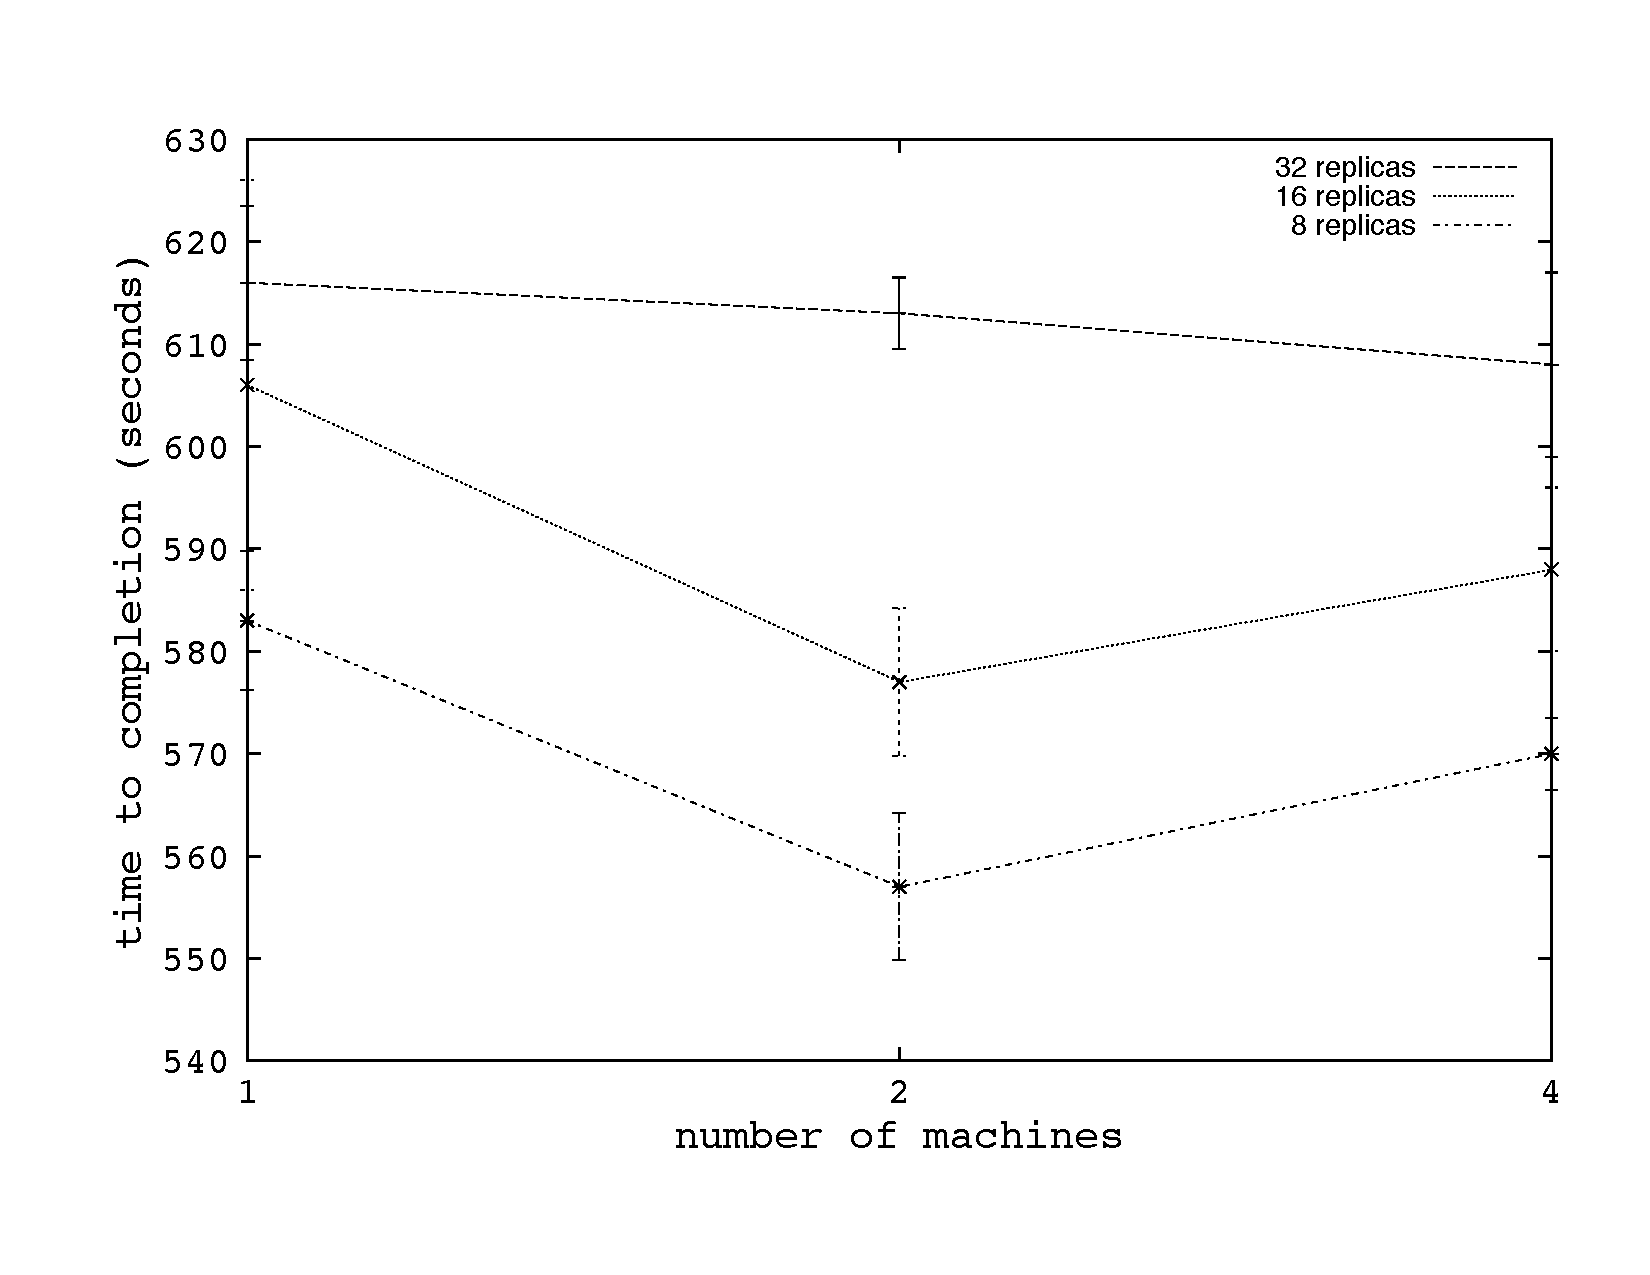
\includegraphics[scale=0.35]{../data/decent_scaleout.pdf}\qquad
%\caption{\textbf{Scale-out performance for 8, 16 and 32 replicas, asynchronous (decentralised):}  The experiments were done on LONI resources and repeated at least 5 times. The error bars denote standard error. As the number of machines increases, the time-to-completion remains constant as there are no remote file copies or synchronisation costs.} \alnote{Please insert proper caption}
%\label{fig:scaleout_dec}
%\end{figure}
%
%
%\subsubsection{Scale out - Asynchronous (decentralised)}
%\alnote{This is a very short analysis. I think the decentralised algorithm and thus, less synchronisation
%should also play an important role?}
%{\it Results:} The results are shown in the graph~\ref{fig:scaleout_dec}. We see in the graph that as we go from 1 to 2 and 4 machines, we do not observe a perceptible change in the time to completion.
%The time to completion almost stays constant from 1 machine to 2 and 4 machines. We believe that this is due to the fact that there is no remote file staging involved in this implementation. The fact that this is the asynchronous RE algorithm and a decentralised implementation also play a role. There is no synchronisation involved in this implementation. 

% Since replicas are currently started sequentially by the master, a
% delay between the start and thus the termination of the first and last
% replica exists.
% From table1\ref{}, it can be seen that in synchronous RE, the largest
% component causing slow down is $T_W$. 
% (number of pairwise
% exchanges) increases, while
% Thus by substituting the values from the table in the
% eqn2.2, and changing $N_X$, we can understand how the values in graph1
% are possible.

% In the asynchronous (decentralized) RE, as can be seen from the
% table1\ref{}, the individual values for each of the components that
% make up the time to make a pairwise exchange are not smaller. In fact,
% $T_X$ is very large when compared to other cases. 

% In contrast to the other cases, the exchanges are performed by the
% replica-agents instead of having the RE-Manager make the exchanges
% centrally (\jhanote{or serially}).  Thus finding a partner -- and thus
% $T_f$, has two components: a search and reverify stage, which must
% both be successful before an exchange is carried out.
% %a successful search and reverify stage.

% When searching for a replica randomly, on average it takes $N_R \over
% 2$ attempts to find a replica that is in the \texttt{done} state.
% However, finding a replica in the \texttt{done} state is not enough to
% ensure an exchange attempt.  Given that there are several ``active
% exchanges'' being attempted, often the reverify step leads to an
% aborted exchange attempt; a reverify step must occur to ensure there
% has been no change in the states of either of the two replicas
% involved.  The exact number is a random variable, determined by the
% number of replicas, the distribution of states and whether the attempt
% to find a replica is random or sequential. Empirical observation
% suggests that between 2-5 find and reverify attempts before an
% exchange is attempted.  But in general, replicas contend with each
% other to lock a partner for exchange; this gets worse with increasing
% number of replicas, i.e., $T_f$ increases with increasing $N_R$.
% Specifically, for the random access case, we find $T_f$ is $2 \times
% N_R \times 0.1$ (where $0.1$ is the typical time to set/get a value
% to/from the advert server)

% and for the sequential access case, we find
% $T_f$ is $2.5 \times N_R \times 0.11$. 
% We implemented a serial search
% for upto 32 replicas, and a random search for $N_R$ value greater than
% 32.
% and from 64 to 256 replicas we implemented a random search. 
%\alnote{in the centralised as well, doesn't it?} 
% For the random access case,\alnote{I think in sec 4 we only talk about
%   the random case now} 


% On average per exchange involving two replicas, one of the necessary input 
% file transfers involves a remote copy, i.\,e.\ for 32 exchanges, 32 remote 
% transfers are necessary. Thus, the additional overhead in $T_{file}$ can be 
% approximated to $0.37 \times 32=12\,s$. Within error bars, this is the 
% difference we see in the
% Figure~\ref{fig:scaleout_cent} when moving from 1 to 2 machines in the 8
% replica configuration. 

% We do not have an accurate explanation for the behaviour of the 16 and
% 32 replica configurations. 



